% RQ2 paper: from requirement atoms to a DCAT-AP extension.
% Companion of the RQ1 paper (ESWC 2027 submission); same skeleton, same voice.
% Build: see paper/README.md (latexmk -pdf main.tex). Class: Springer LNCS (llncs).
\documentclass[runningheads]{llncs}

\usepackage[T1]{fontenc}
\usepackage{graphicx}
\usepackage{booktabs}
\usepackage{multirow}
\usepackage{array}
\usepackage{amsmath}
\usepackage{amssymb}
\usepackage{xcolor}
\usepackage{xspace}
\usepackage{tikz}
\usetikzlibrary{positioning,arrows.meta,fit,calc,backgrounds}
\usepackage{acronym}
\usepackage[hidelinks]{hyperref}

% Draft markers, in the style of the RQ1 draft ("[TODO: ...]"). Search the source for \todo and \verify.
\newcommand{\todo}[1]{\textcolor{red}{\textbf{[TODO: #1]}}}
\newcommand{\verify}[1]{\textcolor{red}{\textbf{[verify: #1]}}}
% Vocabulary terms and identifiers (prefixed names, check ids).
\newcommand{\term}[1]{\texttt{#1}}

% Acronyms (acronym package), defined without printing a list.
% The expansions follow the first uses in the RQ1 paper (PDF of 13 November 2026);
% verify the keys against the RQ1 main.tex when it is available.
% Use \ac{} in running text, \acp{} for plurals, \acs{} for the short form only.
\acrodef{AI}{artificial intelligence}
\acrodef{API}{application programming interface}
\acrodef{DCAT}{Data Catalog Vocabulary}
\acrodef{DCAT-AP}{DCAT Application Profile for data portals in Europe}
\acrodef{DQV}{Data Quality Vocabulary}
\acrodef{DSV}{Data Specification Vocabulary}
\acrodef{EHDS}{European Health Data Space}
\acrodef{FAIR}{findable, accessible, interoperable and reusable}
\acrodef{IRI}{Internationalized Resource Identifier}
\acrodef{LinkML}{Linked Data Modeling Language}
\acrodef{LLM}{large language model}
\acrodef{NAPCORE}{National Access Point Coordination Organisation for Europe}
\acrodef{OWL}{Web Ontology Language}
\acrodef{RDF}{Resource Description Framework}
\acrodef{SEMIC}{Semantic Interoperability Community}
\acrodef{SHACL}{Shapes Constraint Language}
\acrodef{VPE}{Visual Profile Editor}

% Generated by paper/scripts/make_pilot_tables.py from paper/inputs/pilot-runs-2026-11-13.md.
% Do not edit by hand. \pilot{case}{run}{field}: case jrc|stat, run rules|run1|run2.
\makeatletter
\newcommand{\pilot}[3]{\@ifundefined{pilot@#1@#2@#3}{\textbf{??}}{\@nameuse{pilot@#1@#2@#3}}}
\newcommand{\pilotkind}[3]{\@ifundefined{pilotkind@#1@#2@#3}{\textbf{??}}{\@nameuse{pilotkind@#1@#2@#3}}}
\@namedef{pilot@jrc@rules@wall}{1}
\@namedef{pilot@jrc@rules@calls}{38}
\@namedef{pilot@jrc@rules@cached}{0}
\@namedef{pilot@jrc@rules@intok}{0}
\@namedef{pilot@jrc@rules@outtok}{0}
\@namedef{pilot@jrc@rules@addressed}{2}
\@namedef{pilot@jrc@rules@partial}{0}
\@namedef{pilot@jrc@rules@pending}{15}
\@namedef{pilot@jrc@rules@unaddressed}{0}
\@namedef{pilot@jrc@rules@covered}{0}
\@namedef{pilot@jrc@rules@included}{2}
\@namedef{pilot@jrc@rules@rejected}{0}
\@namedef{pilot@jrc@rules@needsreview}{14}
\@namedef{pilot@jrc@rules@extrate}{0.000}
\@namedef{pilot@jrc@rules@verdict}{conformant}
\@namedef{pilot@jrc@rules@added}{2}
\@namedef{pilot@jrc@rules@tightened}{0}
\@namedef{pilot@jrc@rules@loosened}{0}
\@namedef{pilot@jrc@rules@warnings}{0}
\@namedef{pilot@jrc@run1@wall}{1018}
\@namedef{pilot@jrc@run1@calls}{83}
\@namedef{pilot@jrc@run1@cached}{2}
\@namedef{pilot@jrc@run1@intok}{133{,}326}
\@namedef{pilot@jrc@run1@outtok}{81{,}993}
\@namedef{pilot@jrc@run1@addressed}{10}
\@namedef{pilot@jrc@run1@partial}{1}
\@namedef{pilot@jrc@run1@pending}{4}
\@namedef{pilot@jrc@run1@unaddressed}{2}
\@namedef{pilot@jrc@run1@covered}{0}
\@namedef{pilot@jrc@run1@included}{12}
\@namedef{pilot@jrc@run1@rejected}{3}
\@namedef{pilot@jrc@run1@needsreview}{5}
\@namedef{pilot@jrc@run1@extrate}{0.364}
\@namedef{pilot@jrc@run1@verdict}{conformant with warnings}
\@namedef{pilot@jrc@run1@added}{8}
\@namedef{pilot@jrc@run1@tightened}{3}
\@namedef{pilot@jrc@run1@loosened}{0}
\@namedef{pilot@jrc@run1@warnings}{1}
\@namedef{pilot@jrc@run2@wall}{461}
\@namedef{pilot@jrc@run2@calls}{74}
\@namedef{pilot@jrc@run2@cached}{30}
\@namedef{pilot@jrc@run2@intok}{65{,}985}
\@namedef{pilot@jrc@run2@outtok}{38{,}247}
\@namedef{pilot@jrc@run2@addressed}{11}
\@namedef{pilot@jrc@run2@partial}{1}
\@namedef{pilot@jrc@run2@pending}{2}
\@namedef{pilot@jrc@run2@unaddressed}{3}
\@namedef{pilot@jrc@run2@covered}{0}
\@namedef{pilot@jrc@run2@included}{13}
\@namedef{pilot@jrc@run2@rejected}{4}
\@namedef{pilot@jrc@run2@needsreview}{3}
\@namedef{pilot@jrc@run2@extrate}{0.417}
\@namedef{pilot@jrc@run2@verdict}{conformant with warnings}
\@namedef{pilot@jrc@run2@added}{9}
\@namedef{pilot@jrc@run2@tightened}{3}
\@namedef{pilot@jrc@run2@loosened}{0}
\@namedef{pilot@jrc@run2@warnings}{1}
\@namedef{pilot@jrc@run3@wall}{1961}
\@namedef{pilot@jrc@run3@calls}{74}
\@namedef{pilot@jrc@run3@cached}{1}
\@namedef{pilot@jrc@run3@intok}{122{,}356}
\@namedef{pilot@jrc@run3@outtok}{76{,}346}
\@namedef{pilot@jrc@run3@addressed}{8}
\@namedef{pilot@jrc@run3@partial}{0}
\@namedef{pilot@jrc@run3@pending}{4}
\@namedef{pilot@jrc@run3@unaddressed}{5}
\@namedef{pilot@jrc@run3@covered}{0}
\@namedef{pilot@jrc@run3@included}{8}
\@namedef{pilot@jrc@run3@rejected}{4}
\@namedef{pilot@jrc@run3@needsreview}{4}
\@namedef{pilot@jrc@run3@extrate}{0.571}
\@namedef{pilot@jrc@run3@verdict}{conformant with warnings}
\@namedef{pilot@jrc@run3@added}{5}
\@namedef{pilot@jrc@run3@tightened}{2}
\@namedef{pilot@jrc@run3@loosened}{0}
\@namedef{pilot@jrc@run3@warnings}{1}
\@namedef{pilot@stat@rules@wall}{1}
\@namedef{pilot@stat@rules@calls}{32}
\@namedef{pilot@stat@rules@cached}{0}
\@namedef{pilot@stat@rules@intok}{0}
\@namedef{pilot@stat@rules@outtok}{0}
\@namedef{pilot@stat@rules@addressed}{2}
\@namedef{pilot@stat@rules@partial}{1}
\@namedef{pilot@stat@rules@pending}{11}
\@namedef{pilot@stat@rules@unaddressed}{0}
\@namedef{pilot@stat@rules@covered}{0}
\@namedef{pilot@stat@rules@included}{2}
\@namedef{pilot@stat@rules@rejected}{0}
\@namedef{pilot@stat@rules@needsreview}{11}
\@namedef{pilot@stat@rules@extrate}{0.000}
\@namedef{pilot@stat@rules@verdict}{conformant}
\@namedef{pilot@stat@rules@added}{}
\@namedef{pilot@stat@rules@tightened}{1}
\@namedef{pilot@stat@rules@loosened}{0}
\@namedef{pilot@stat@rules@warnings}{0}
\@namedef{pilot@stat@run1@wall}{892}
\@namedef{pilot@stat@run1@calls}{64}
\@namedef{pilot@stat@run1@cached}{0}
\@namedef{pilot@stat@run1@intok}{105{,}086}
\@namedef{pilot@stat@run1@outtok}{67{,}732}
\@namedef{pilot@stat@run1@addressed}{7}
\@namedef{pilot@stat@run1@partial}{0}
\@namedef{pilot@stat@run1@pending}{1}
\@namedef{pilot@stat@run1@unaddressed}{6}
\@namedef{pilot@stat@run1@covered}{0}
\@namedef{pilot@stat@run1@included}{9}
\@namedef{pilot@stat@run1@rejected}{8}
\@namedef{pilot@stat@run1@needsreview}{1}
\@namedef{pilot@stat@run1@extrate}{0.857}
\@namedef{pilot@stat@run1@verdict}{conformant with warnings}
\@namedef{pilot@stat@run1@added}{6}
\@namedef{pilot@stat@run1@tightened}{}
\@namedef{pilot@stat@run1@loosened}{0}
\@namedef{pilot@stat@run1@warnings}{1}
\@namedef{pilot@stat@run2@wall}{482}
\@namedef{pilot@stat@run2@calls}{64}
\@namedef{pilot@stat@run2@cached}{20}
\@namedef{pilot@stat@run2@intok}{67{,}528}
\@namedef{pilot@stat@run2@outtok}{39{,}879}
\@namedef{pilot@stat@run2@addressed}{10}
\@namedef{pilot@stat@run2@partial}{0}
\@namedef{pilot@stat@run2@pending}{3}
\@namedef{pilot@stat@run2@unaddressed}{1}
\@namedef{pilot@stat@run2@covered}{0}
\@namedef{pilot@stat@run2@included}{11}
\@namedef{pilot@stat@run2@rejected}{3}
\@namedef{pilot@stat@run2@needsreview}{4}
\@namedef{pilot@stat@run2@extrate}{0.556}
\@namedef{pilot@stat@run2@verdict}{conformant}
\@namedef{pilot@stat@run2@added}{6}
\@namedef{pilot@stat@run2@tightened}{3}
\@namedef{pilot@stat@run2@loosened}{0}
\@namedef{pilot@stat@run2@warnings}{0}
\@namedef{pilot@stat@run3@wall}{1937}
\@namedef{pilot@stat@run3@calls}{57}
\@namedef{pilot@stat@run3@cached}{0}
\@namedef{pilot@stat@run3@intok}{90{,}564}
\@namedef{pilot@stat@run3@outtok}{61{,}846}
\@namedef{pilot@stat@run3@addressed}{5}
\@namedef{pilot@stat@run3@partial}{2}
\@namedef{pilot@stat@run3@pending}{1}
\@namedef{pilot@stat@run3@unaddressed}{5}
\@namedef{pilot@stat@run3@covered}{1}
\@namedef{pilot@stat@run3@included}{7}
\@namedef{pilot@stat@run3@rejected}{7}
\@namedef{pilot@stat@run3@needsreview}{3}
\@namedef{pilot@stat@run3@extrate}{0.500}
\@namedef{pilot@stat@run3@verdict}{conformant with warnings}
\@namedef{pilot@stat@run3@added}{5}
\@namedef{pilot@stat@run3@tightened}{}
\@namedef{pilot@stat@run3@loosened}{0}
\@namedef{pilot@stat@run3@warnings}{1}
\@namedef{pilotkind@jrc@run1@reuse}{4}
\@namedef{pilotkind@jrc@run1@refine}{3}
\@namedef{pilotkind@jrc@run1@mintproperty}{4}
\@namedef{pilotkind@jrc@run1@mintclass}{1}
\@namedef{pilotkind@jrc@run2@reuse}{4}
\@namedef{pilotkind@jrc@run2@refine}{3}
\@namedef{pilotkind@jrc@run2@mintproperty}{5}
\@namedef{pilotkind@jrc@run2@mintclass}{1}
\@namedef{pilotkind@jrc@run3@reuse}{1}
\@namedef{pilotkind@jrc@run3@refine}{2}
\@namedef{pilotkind@jrc@run3@mintproperty}{4}
\@namedef{pilotkind@jrc@run3@mintclass}{1}
\@namedef{pilotkind@stat@run1@reuse}{0}
\@namedef{pilotkind@stat@run1@refine}{1}
\@namedef{pilotkind@stat@run1@mintproperty}{6}
\@namedef{pilotkind@stat@run1@mintclass}{2}
\@namedef{pilotkind@stat@run2@reuse}{1}
\@namedef{pilotkind@stat@run2@refine}{3}
\@namedef{pilotkind@stat@run2@mintproperty}{5}
\@namedef{pilotkind@stat@run2@mintclass}{2}
\@namedef{pilotkind@stat@run3@reuse}{2}
\@namedef{pilotkind@stat@run3@refine}{1}
\@namedef{pilotkind@stat@run3@mintproperty}{3}
\@namedef{pilotkind@stat@run3@mintclass}{1}
\makeatother


\begin{document}

\title{TITLE}
\titlerunning{RUNNING TITLE}
\author{Anonymous Author(s)}
\authorrunning{Anonymous Author(s)}
\institute{Anonymous Institution}

\maketitle

\begin{abstract}
\todo{abstract}
\keywords{DCAT-AP \and Application profiles \and LLMs}
\end{abstract}

\acresetall
% Introduction (outline brief 6.1; mirrors RQ1 L35-102, seven paragraphs to seven). The abstract expands DCAT,
% DCAT-AP and LLM as RQ1's does; \acresetall expands them again here (verify, not printed: RQ1 main.tex convention,
% readme-notes question 1). Describes the tool at 5ffd56e (DCAT-state pinning, rebase). No development-run number.
\section{Introduction}\label{sec:intro}

The W3C \ac{DCAT} is a vocabulary for interoperability between data catalogs~\cite{w3cdcat3}, and the
\ac{DCAT-AP} adds obligations, cardinalities and controlled vocabularies~\cite{semicdcatap}. Domain extensions
build on \acs{DCAT-AP} and inherit its classes, properties and obligations: GeoDCAT-AP and StatDCAT-AP for
geospatial and statistical data~\cite{geodcatap10,statdcatap}, mobilityDCAT-AP for mobility
data~\cite{scrocca2025mobilitydcat}, HealthDCAT-AP for the \ac{EHDS}~\cite{derycke2025healthdcat} and DCAT-AP-JRC
for research data~\cite{perego2016jrc}. What an extension adds is a set of changes to its base: existing
properties used where the base states nothing, base constraints tightened and terms minted in the extension's own
namespace~\cite{semicreuse2026}.
% src for the three kinds of change: @5ffd56e docs/conformance.md:12-14, :45 (RG lines 376-379, 471-474)

Defining such an extension is a requirements problem before it is a modeling problem~\cite{anon2027rq1}; once
the requirements are settled, it is a modeling problem under the constraints the base imposes. A requirement is
met by the base as it stands, by a tightened base constraint, by a reused term or by a new one; mobilityDCAT-AP,
for example, makes the update frequency mandatory where its base has it optional~\cite{mobilitydcatspec}.
% src: RQ1 L59-61 (the companion's own example)
\todo{author: keep the companion's mobilityDCAT-AP example (a test case) or use the generic wording ``raising an
optional property to mandatory'' (Q17)}
The guidance of the \ac{SEMIC} orders these choices, rules out loosening a base constraint, ``as the result would
no longer be compliant with DCAT-AP'', and expects use cases to justify new elements and tightened
constraints~\cite{semicreuse2026}. \verify{verbatim against the guidelines}
% src: @5ffd56e docs/conformance.md:12-14 (RG lines 376-379) and :47 (RG lines 262-264)
The base itself profiles a DCAT version as it stood when the release was made: \acs{DCAT-AP}~1.1 builds on % src: @5ffd56e B/data/base-profiles/dcat-ap-1.1/profile.yaml:33
DCAT~2014 and \acs{DCAT-AP}~3.0.1 on DCAT~3. \verify{release quotes} % src: @5ffd56e B/data/base-profiles/dcat-ap-3.0.1/profile.yaml:43

Existing authoring tools and generators help with the modeling, not with this derivation
(Sect.~\ref{sec:related}). Dataspecer generates \ac{DSV} and \ac{SHACL} from profiles of profiles that people
author \verify{new bib entry: Dataspecer}, but in a reading of its code it uses no language model and does not
check that a profile refines its base; generators based on \acp{LLM} write ontologies from competency questions or
relational schemas~\cite{lippolis2025ontology,fathallah2026rigor}, and shape generators are given the
terms \verify{new bib entry: NL2SHACL-Bench}. Of those we examined, none derives an extension of a pinned base
release from requirements and records, for every element, the requirement it serves and the base value it
changes. \verify{each ``none'' claim}
% src: docs/research/B1-dataspecer.md:29 (finding 7: no refinement check); visual-profile-editor
% docs/dataspecer-spike.md:9-30, 67-75 (SHACL from profiles; no LLM features, medium confidence: code reading only)

Such records are needed after the first release too, because a base does not stand still. \acs{DCAT-AP}~3.0.1
relaxed three cardinalities of 3.0.0 \verify{new bib entry: DCAT-AP 3.0.1}, and 68 issues on \acs{DCAT-AP}, % src: @5ffd56e docs/conformance.md:22-23 (three cardinalities, from the 3.0.1 CHANGELOG); RQ1 L71-73 (68 issues)
StatDCAT-AP and GeoDCAT-AP were reviewed for maintenance in less than nine months~\cite{dragan2019maintenance}. % src: RQ1 L71-73
\verify{3.0.1 CHANGELOG}
When the base moves to another release, and possibly to another DCAT version, an extension has to find the elements
that rest on what changed, and a profile that names neither the requirement behind an element nor the base value
it tightened cannot show it. With such a record, the rebase of Sect.~\ref{sec:impl} compares each change under
the old and the new base.
% src: @5ffd56e B/engine/rebase.py:73-180; B/engine/pipeline.py:557-609; docs/dcat-versions.md:185-210

This paper addresses the gap with a pipeline in which an \acs{LLM} acts as a bounded decider: for each
requirement atom it decides whether the base already meets it and otherwise fills typed change records from
retrieved candidate terms, while program code mints identifiers and compiles the extension. Four pillars shape % src: @5ffd56e docs/design.md:5-10 (the design goals; outline section 2)
the design: (1)~reuse first and minimal, (2)~traced, with an obligation the atom's wording licenses,
(3)~decided by the model, with the final say for a person and every step open to inspection, and
(4)~conformant to the base; Sect.~\ref{sec:problem} turns them into the criteria E1--E4. The companion workflow
ends with needs that cite their passages; this pipeline starts from atoms and ends with changes that cite them,
each with a verbatim quote of its atoms, the base value beside each new one and the decisions behind it, so that
when an atom or the base changes a reviewer can find the changes that rest on it. Program code checks every
change and the compiled extension, a model only judges whether the atoms support a change, and only a person
releases the extension; automatic acceptance is a decision policy, not a claim that the checks establish
correctness.
% src: @5ffd56e B/engine/prompts.py:24-72; B/engine/verify.py:482-483; B/engine/pipeline.py:221-267, 611-640;
% docs/design.md:14-31

We ask, for the modeling part of profile engineering: \emph{How much of what a published DCAT-AP extension adds
to its base does a pipeline reconstruct from the requirement atoms behind it that reuses before it mints and
keeps every change reviewable from the atoms it covers, its relation to the base and its decisions, while the
extension stays conformant to the base, and what do retrieval, repair and the judge contribute?} We compare the
full pipeline with a rules baseline and a closed-book model, and remove retrieval, repair and the judge in turn.
\todo{conditions: final set (Q7)}
% src: @5ffd56e B/contracts.py:592-596 (the switches retrieval, repair_rounds, attribution_check)

This paper makes three contributions:
\begin{itemize}
\item a formulation of an extension as a justified delta over a pinned \acs{DCAT-AP} release and the DCAT version
  it builds on, with six change kinds, a justification contract and a legal-refinement order, and a pipeline that % src: @5ffd56e B/contracts.py:39-46 (ChangeKind)
  implements it, grounded step by step in requirements-engineering and ontology-generation work
  (Sects.~\ref{sec:problem} and~\ref{sec:pipeline});
\item reference deltas for the five published extensions of the companion benchmark, defined as each published % src: RQ1 L381-388
  profile minus its base and matched to the generated changes element by element (Sect.~\ref{sec:benchmark});
  \todo{reference deltas: build, align and freeze before this claim stands}
\item an evaluation design in two views, how much of the reference delta the output recovers and how much of the
  output the reference accounts for, with reuse, conformance, review load and cost (Sects.~\ref{sec:setup}
  and~\ref{sec:results}). \todo{switch ``an evaluation design'' to ``an evaluation'' when results exist}
\end{itemize}

\section{Related Work}
\todo{section to be written}

\section{PROBLEM}
\todo{section to be written}

% Sect. 4 Pipeline (outline brief 6.4). Describes the tool at commit 5ffd56e of the main branch ("Work inside the
% DCAT state each DCAT-AP release builds on; keep all versions; rebase"), which is not merged into the paper branch
% (TODO in Sect. 4.4). In the src comments, B = backend/profile_extensioner at 5ffd56e; CONF5, DCS, ENG, ISS, KCU,
% LIT, LITD are the outline's shorthands (docs/conformance.md at 5ffd56e; scratchpad digests dcat-state, engine,
% issues-at-main, knowledge-compile-ui; docs/literature-steps.md; literature digest). Mirrors RQ1 Sect. 4
% (L236-355): intro, Fig. 1, three subsections that follow the rows of the figure, then the implementation.
\section{Pipeline}\label{sec:pipeline}

\begin{figure}[t]
  \centering
  % Fig. 1: the pipeline of the tool at commit 5ffd56e. Mirrors the RQ1 paper's Fig. 1: numbered operations in three
% labelled rows, the middle row read from right to left. Encoding in RQ1's grammar: dashed border = the operation
% calls the model (3 proposer, 4 judge, 5 repairer); light fill = a person decides (9); plain = program code. The
% blackboard band is program code as well, so it has a plain (solid, grey) border.
% Sources of the labels: B/engine/intake.py, retrieve.py, propose.py, verify.py (V1-V5, D1-D3, T1, B1),
% pipeline.py (T2 judge, repair, consolidation, decision, sign-off), compile/, conformance/check.py (C1-C8)
% at 5ffd56e; B = backend/profile_extensioner.
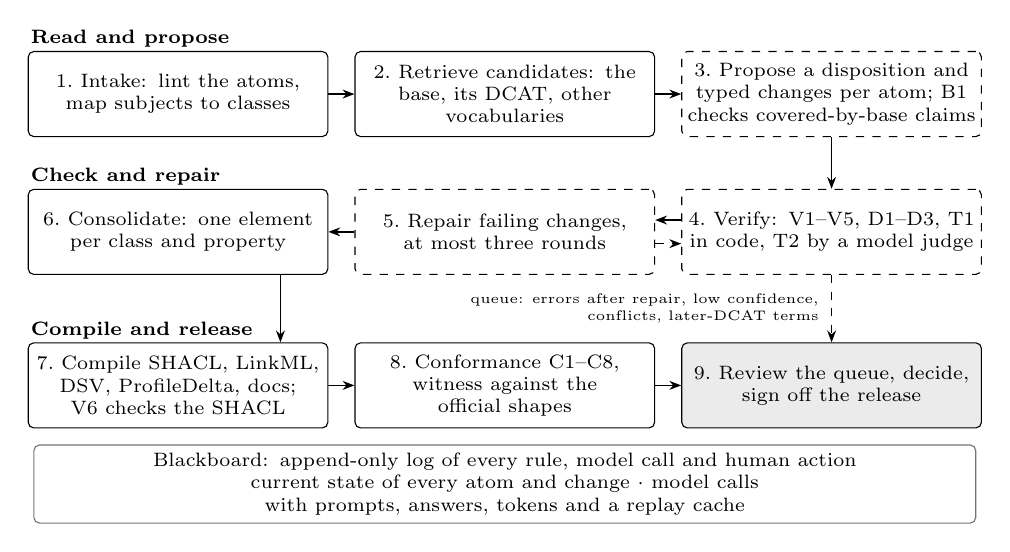
\begin{tikzpicture}[
    font=\scriptsize,
    op/.style={draw, rounded corners=2pt, minimum height=1.08cm, align=center,
               inner sep=1.5pt, text width=3.7cm},
    llm/.style={op, dashed},
    human/.style={op, fill=black!8},
    row/.style={font=\scriptsize\bfseries, anchor=south west, inner sep=1pt},
    flow/.style={-{Stealth[length=1.5mm]}, semithick},
    side/.style={-{Stealth[length=1.5mm]}, semithick, dashed},
  ]
  % row 1: read and propose (left to right)
  \node[op]  (o1) at (0,0)     {1.\ Intake: lint the atoms,\\ map subjects to classes};
  \node[op]  (o2) at (4.15,0)  {2.\ Retrieve candidates: the\\ base, its DCAT, other\\ vocabularies};
  \node[llm] (o3) at (8.3,0)   {3.\ Propose a disposition and\\ typed changes per atom; B1\\ checks covered-by-base claims};
  % row 2: check and repair (right to left)
  \node[llm] (o4) at (8.3,-1.75)  {4.\ Verify: V1--V5, D1--D3, T1\\ in code, T2 by a model judge};
  \node[llm] (o5) at (4.15,-1.75) {5.\ Repair failing changes,\\ at most three rounds}; % src: @5ffd56e B/contracts.py:595
  \node[op]  (o6) at (0,-1.75)    {6.\ Consolidate: one element\\ per class and property};
  % row 3: compile and release (left to right)
  \node[op]    (o7) at (0,-3.7)    {7.\ Compile SHACL, LinkML,\\ DSV, ProfileDelta, docs;\\ V6 checks the SHACL};
  \node[op]    (o8) at (4.15,-3.7) {8.\ Conformance C1--C8,\\ witness against the\\ official shapes};
  \node[human] (o9) at (8.3,-3.7)  {9.\ Review the queue, decide,\\ sign off the release};
  % row labels
  \node[row] at (o1.north west) {Read and propose};
  \node[row] at (o6.north west) {Check and repair};
  \node[row] at (o7.north west) {Compile and release};
  % flow
  \draw[flow] (o1) -- (o2);
  \draw[flow] (o2) -- (o3);
  \draw[flow] (o3) -- (o4);
  \draw[flow] ([yshift=1.5mm]o4.west) -- ([yshift=1.5mm]o5.east);
  \draw[side] ([yshift=-1.5mm]o5.east) -- ([yshift=-1.5mm]o4.west);
  \draw[flow] (o5) -- (o6);
  \draw[flow] ([xshift=13mm]o6.south) -- ([xshift=13mm]o7.north);
  \draw[flow] (o7) -- (o8);
  \draw[flow] (o8) -- (o9);
  \draw[side] (o4.south) -- node[left=1pt, font=\tiny, align=right] {queue: errors after repair, low confidence,\\
    conflicts, later-DCAT terms} (o9.north);
  % blackboard (program code: plain border)
  \node[draw=black!55, rounded corners=2pt, anchor=north, text width=11.75cm, align=center,
        inner sep=3pt] (bb) at (4.15,-4.45)
        {Blackboard: append-only log of every rule, model call and human action\\
         current state of every atom and change\ $\cdot$\ model calls with prompts, answers, tokens and a replay cache};
\end{tikzpicture}

  \caption{The pipeline. Dashed operations call the model; with the rules baseline, offline rules take their place
    (Sect.~\ref{sec:setup}). Light: the person's operation. A change that fails a check at error level goes to
    repair~(5), at most three rounds, and, still failing, to the review queue~(9), as do conflicts, changes below % src: @5ffd56e B/contracts.py:595 (repair_rounds 3); B/engine/pipeline.py:246-267, 295-338, 347-353
    the confidence threshold and, by default, changes that use a term of a later \acs{DCAT}. Proposer, repairer and judge use the
    same model, so the judge is not independent of the proposer.}
  \label{fig:pipeline}
\end{figure}

Figure~\ref{fig:pipeline} shows the nine operations in three rows: the model acts as proposer~(3), judge~(4) and % src: paper/figures/pipeline.tex (nodes o1-o9, three rows); @5ffd56e B/contracts.py:104-107 (nine stages); B/engine/prompts.py:1 (three roles)
repairer~(5), a person decides in the last~(9), and program code does the rest. The supplementary material follows % src: paper/figures/pipeline.tex (operation numbers 3, 4, 5, 9)
one atom of a synthetic demo through them.
\todo{supplementary material: one atom of the synthetic demo through the nine operations}
The pipeline also runs without a model, with offline rules in the dashed operations (Sect.~\ref{sec:setup}). % src: @5ffd56e B/llm/mock.py:1-10

\subsection{Read and propose}\label{sec:read}

Intake checks the form of every atom (Sect.~\ref{sec:problem}) without rewriting it and maps its subject to a % src: @5ffd56e B/engine/intake.py:1-7, 108-131
class of the base. An \ac{IRI} or a prefixed name in the statement is an error, and the atom stays unclear % src: @5ffd56e B/engine/intake.py:39-51, 115-116; B/engine/pipeline.py:184-185
without a proposal; a subject that is not a plain word, a very short statement, a compound statement and a % src: @5ffd56e B/engine/intake.py:52-87 (warnings; vague words and an unspecified modality are info)
modality the wording contradicts are warnings, the last two adapted from characteristics of a well-formed % LIT G2-S02 (partial, Ours): compound = singular, modality mismatch = unambiguous
requirement \cite{iso29148}.

Retrieval is deterministic: a field-weighted lexical score, without embeddings. The base's elements on the atom's % src: @5ffd56e B/knowledge/vocab_index.py:8, 332-343, 352-367 (label 3, local name 2, definition 1; idf); KCU §2.4
class are boosted and, when they match reasonably, listed first; properties that the base's \acs{DCAT} lists for % src: @5ffd56e B/engine/retrieve.py:40, 52, 108-132, 259-263 (BASE_FIRST_SHARE 0.35)
the class but the base does not profile are boosted ($\times$1.4; the 1.x bases have none); terms that only a later % src: @5ffd56e B/engine/retrieve.py:41, 134-156; DCS §2.4 (rung 2 empty for 1.x)
\acs{DCAT} defines are marked with their version and down-weighted ($\times$0.5), and terms the base deprecates % src: @5ffd56e B/engine/retrieve.py:42, 82-88; B/engine/prompts.py:136-138
and vocabularies made for one domain are down-weighted too. % src: @5ffd56e B/engine/retrieve.py:43, 47-49, 186-190

The proposer is called once per atom, without the other atoms' changes, and fills a typed record by a numbered % src: @5ffd56e B/engine/pipeline.py:188-191 (no pending changes passed); ISS E7.2
procedure: it restates the information needed, fixes the class and walks the ladder of E1 from the base slice to a % src: @5ffd56e B/engine/prompts.py:30-48
mint, taking a later-\acs{DCAT} term only when no other term carries the information and minting only after saying why each plausible
candidate fails; every constraint needs a reason, and the answer a confidence. Program code then builds the change
records of Sect.~\ref{sec:problem}, and a refinement inherits from the base what it leaves unset, except the % src: @5ffd56e B/engine/propose.py:175-306 (unchanged since 2b92d77, ISS header)
obligation. B1 checks each covered-by-base claim as E1 requires, and a failed claim leaves the atom unclear. % src: @5ffd56e B/engine/verify.py:513-533; B/engine/pipeline.py:200-211
One atom per memoryless call that first asks whether the base already meets it follows the released Memoryless % LIT G1-S03 (Ours: the merge), G1-S05
CQbyCQ prompt \cite{lippolis2025ontology}, and reuse limited to retrieved terms follows RIGOR's released % LIT G1-S08
implementation \cite{fathallah2026rigor}; the ladder is our reading of SEMIC's guidance \cite{semicreuse2026}. Here the model % LIT G3-S01 (implemented, Ours)
chooses the properties, within typed records, and never writes \ac{SHACL} or mints an identifier.

\subsection{Check and repair}\label{sec:check}

Program code checks every change in a fixed order (Table~\ref{tab:checks} in the appendix): V1 term existence, V2 % src: @5ffd56e B/engine/verify.py:3-18, 166-211, 482-483; ISS E7.1 (union domains fixed)
domain and range, union domains included, D1 to D3 the \acs{DCAT} state, V3 legal refinement, V4 reuse before mint,
V5 consistency and T1 the trace; a set-level V5 error marks every live change on the same class and property. % src: @5ffd56e B/engine/verify.py:493-510
By default a term that only a later \acs{DCAT} defines gives a D1 warning that sends the change to a person; a % src: @5ffd56e B/contracts.py:604-606 (later_dcat_terms review|forbid|allow); B/engine/verify.py:228-242
term only an earlier \acs{DCAT} defines and a \acs{DCAT} property without a declared domain on a class the base's % src: @5ffd56e B/engine/verify.py:243-245, 259-273
\acs{DCAT} does not list it for are D1 errors, terms the base's \acs{DCAT} or the base deprecates are D2 errors, % src: @5ffd56e B/engine/verify.py:246-257
and D3 warns on every use of the six inverse properties in the \acs{DCAT} namespace. Only a change without an % src: @5ffd56e B/engine/verify.py:274-280; DCS §2.6 (11 DCAT 3 pairs, 5 outside the dcat: namespace)
error reaches the judge T2, which is told to judge from the atoms as written, not from published profiles: % src: @5ffd56e B/engine/pipeline.py:279-282; B/engine/prompts.py:84-94
supported passes, unsupported or a named unsupported constraint is an error, and partially supported or an
unavailable judge is a warning. We adapt checking before judging from the released code of a recent blackboard orchestration % src: @5ffd56e B/engine/pipeline.py:221-244; LIT G4-S04 (Ours)
of \acp{LLM} \cite{chmielewski2026blackboard}\verify{chmielewski2026blackboard: known from its released code only;
the entry has no DOI or URL}, and make a missing trace an error where RIGOR's released implementation warns % LIT G1-S18 (Ours)
\cite{fathallah2026rigor}.

A change with an error goes to repair, at most three rounds, scoped to its failed checks as in the released code % src: @5ffd56e B/contracts.py:595; B/engine/pipeline.py:295-338; B/engine/prompts.py:238-242
of RIGOR and IDEA2 \cite{fathallah2026rigor,alharbi2027idea2}: the repairer revises % LIT G1-S13; G2-S13
it, and the new version is verified, judged and decided again, or withdraws it. Consolidation then merges % src: @5ffd56e B/engine/pipeline.py:311-333
compatible changes on one class and property, with the strongest obligation and the tightest bounds, and queues
incompatible ones as a conflict. A change is auto-accepted when no check failed at error level, automatic % src: @5ffd56e B/engine/consolidate.py:25-95 (unchanged since 2b92d77); B/engine/pipeline.py:340-366
acceptance is on, its self-reported confidence is at least 0.5, a majority agrees if there are several votes, and % src: @5ffd56e B/engine/pipeline.py:246-267; B/contracts.py:598-599
no D1 warning asks for a person; otherwise it waits for review. Other warnings never block, and the threshold is % LITD §7 (no cited work supports self-reported confidence as calibrated)
our setting.
\todo{tool: state or fix: duplicates on one class and property go to repair before consolidation would merge them;
a change cleared by consolidation is decided without a judge verdict on its merged atoms (ENG §7.2-7.3; ISS E7.2,
E7.3; Q22)}

\subsection{Compile and release}\label{sec:compile}

Only included changes compile, into seven artifacts. The \ac{SHACL} delta holds only what the extension adds or % src: @5ffd56e B/compile/model.py:47-49; B/engine/pipeline.py:382-392 (seven artefacts)
tightens, with a separate \term{sh:minCount}~1 shape at Warning for a recommended property and, on each property shape, the reason and % src: @5ffd56e B/compile/shacl.py:3-8, 40-91
a \term{prov:wasDerivedFrom} link per covered atom. Its \term{dcterms:conformsTo} names the dated Recommendation of
the base's \acs{DCAT}, and its \term{owl:imports} names the release page for the % src: @5ffd56e B/compile/shacl.py:33-38
3.0.x bases and is absent for the others, so a validator loads the official shapes itself. The other artifacts % src: @5ffd56e B/data/base-profiles/*/profile.yaml:6 (homepage only for 3.0.0, 3.0.1); ISS K10, K11
are the minted vocabulary, \ac{LinkML} \cite{moxon2026linkml} for a visual profile editor\verify{the LinkML output
is valid LinkML (LinkML tooling not installed) and opens in the profile editor}, a \ac{DSV} profile \cite{klimek2026dsv} that, on a 3.0.1 % src: KCU §3.3-3.4; @5ffd56e B/compile/linkml_dsv.py:37-194
base, profiles the \acs{DSV} of \acs{DCAT-AP}~3.0.1 that Dataspecer generated \cite{klimek2024dataspecer}\verify{import of the DSV % src: @5ffd56e B/data/base-profiles/dcat-ap-3.0.1/dsv-index.json:2-3 (mff-uk DSV, generated by Dataspecer); KCU §3.4
output into Dataspecer}, the ProfileDelta, a trace matrix and documentation.

Eight rules then test what E4 asks: C1 legal refinement, C2 joint satisfiability, C3 % src: @5ffd56e B/conformance/check.py:5-21, 111-177, 250-266; CONF5:41-51
and C4 the minted and reused terms, C5 the trace, C6 \acs{SHACL} validity, which V6 already logs at compilation \cite{w3cshacl}, C7 a witness, and C8
the \acs{DCAT} state, failing on a deprecated or removed \acs{DCAT} term and warning on a later one. C7 builds an % src: @5ffd56e B/conformance/check.py:64-99
instance of each constrained class with a value for every required property and validates it with pySHACL % src: @5ffd56e B/conformance/check.py:181-247 (min count >= 1, :204-209; inference "none", :225); KCU §4.3
\cite{sommer2026pyshacl}, without inference,
against base and extension and against the base alone, warning when no valid witness results
(Sect.~\ref{sec:discussion}). The verdict is non-conformant when a rule fails at error level and conformant with % src: @5ffd56e B/conformance/check.py:264-266
warnings when only C7 or C8 warn.

The run stops at the review queue of waiting changes and conflicts: a person can accept,
reject, set back to undecided or edit any change and override any atom's disposition, and release requires an % src: @5ffd56e B/engine/pipeline.py:493-555
empty queue, a current conformance report that is not non-conformant and a recorded sign-off with a hash of the
included changes. An edit is a new version, verified and recorded as accepted; no later machine stage overwrites a % src: @5ffd56e B/engine/pipeline.py:611-635, 512-536
person's decision, and any later decision withdraws the sign-off. Each machine decision is shown with its % src: @5ffd56e B/engine/pipeline.py:115-126, 246-248, 283-285, 301-303, 637-638; ENG §4
evidence, against the over-trust in suggestions reported for OE-Assist \cite{lippolis2025oeassist}. % LIT G1-S16
\todo{tool: state or fix: unclear and unaddressed atoms never enter the queue and do not block the sign-off
(ENG §7.11; ISS E7.11; Q22)}

\subsection{Implementation and traceability}\label{sec:impl}

The pipeline runs in an open research workbench (Fig.~\ref{fig:workbench} in the appendix), where any stage can % src: @5ffd56e frontend/src/App.tsx:203-207, 241, 302; KCU §7
run alone and every intermediate result is on screen. An append-only SQLite blackboard records what every rule, model and
person did, each model call with its prompts, answer and tokens, and serves a replay cache; % src: @5ffd56e B/store/blackboard.py:1-11, 341-351; B/llm/client.py:1-12; KCU §5.3-5.4
the stages cooperate only through it, as the knowledge sources of Hearsay-II do % LIT G4-S01
\cite{erman1980hearsay,nii1986blackboard}, though in a fixed order. The trace matrix shows completeness, not correctness. The official % src: KCU §3.6
files of the nine \acs{DCAT-AP} releases with \acs{SHACL}, 1.1 to 3.0.1, and of \acs{DCAT}~2014, 2 and 3 are kept % src: DCS §1.1, §3; paper/inputs/tool-facts-main-5ffd56e.txt:6-14 (nine bases)
unmodified, with hashes\verify{1.1 and 1.2 record only the hash of the % src: DCS §1.1
zip file}; the 98 tests never call a model.\verify{98 tests pass at the frozen commit} % src: paper/inputs/tool-facts-main-5ffd56e.txt:24 (98 collected)

When the base release changes, a rebase moves the extension onto another release and its \acs{DCAT}: every change
is compared under both bases, human decisions stay, machine changes with a finding that asks for a decision are % src: @5ffd56e B/engine/rebase.py:73-180; B/engine/pipeline.py:557-609
flagged for review, and the extension is checked again, which withdraws the sign-off.
\todo{tool: the consolidation that follows a rebase re-decides flagged machine changes, and a lost covered-by-base
claim is reported but not re-proposed (ISS NEW-1, NEW-2; Q22)}
\todo{described commit: 5ffd56e, not yet in the paper branch (Q14)}

We took the design from 99 steps that we extracted from related work and fact-checked against their released % src: docs/literature-steps.md:3, 6
code, prompts, slides and specifications, some only against abstracts; 33 are implemented, 30 in part and 36 % LITD §0 caution 1 (abstract level for several G2 and G4 sources)
planned, and of the 50 from % src: docs/literature-steps.md:6 (33/30/36); G1 rows :12-36 (13 implemented, 9 in part), G2 rows :42-66 (9, 8): 50 steps, 22 and 17
ontology generation and requirements engineering, 22 are implemented and 17 in part (Table~\ref{tab:steps} in the % src: docs/literature-steps.md:12-36, 42-66 (G1 13+9, G2 9+8; recounted, outline 7.1)
appendix). The workbench is available at \todo{anonymized repository link}.

% Sect. 5 Benchmark (outline brief 6.5; mirrors RQ1 Sect. 5: an opening paragraph, then the run-in heads
% "Development and test cases.", "Inputs." (new), "Reference deltas." (RQ1: "Reference sets.") and "Matching.").
% Test cases: nothing beyond what the RQ1 paper reports (names, RQ1 Table 1 values). No base release and no
% reference-profile version is chosen here (Q3). The reference deltas are not built yet: their counts are \res slots.
% Source shorthand in the % src: comments: outline-final.md Sect. 0.1 (B = backend/profile_extensioner/).
\section{Benchmark}\label{sec:benchmark}

The benchmark adds to the five cases of the companion study \cite{anon2027rq1} what each published extension adds
to its base: a \emph{reference delta}, the published profile minus its base (Table~\ref{tab:cases}). % src: RQ1 L358, L381-388 (five cases); PLAN:9-11
Appendix~\ref{app:benchmark} has the cases in full and, in Fig.~\ref{fig:reference}, the path from a published
profile to Recovery. Each case runs against one pinned base release, one of the nine the tool holds
(Sect.~\ref{sec:impl}), and the \ac{DCAT} version it builds on, because a reference delta exists only relative to
one release. % src: FACTS5:15-23 (nine bases); DCS §3
Against \ac{DCAT-AP}~1.1, built on DCAT~2014, which has no data services, the data service that \ac{DCAT-AP}~2.0.0
profiles is an addition. % src: @5ffd56e B/data/base-profiles/dcat-ap-2.0.0/profile.yaml:25-30; B/data/base-profiles/dcat-ap-1.1/profile.yaml:21-25; B/data/dcat/history.json:30-38 (dcat:DataService introduced in dcat-2)
\todo{base and reference version per case (Q3)} Every reference delta is partial (shape constructs the comparison
does not handle, profiles that publish no shapes).

\begin{table}[tb]
\caption{The benchmark cases, test cases above development cases. Base in~\cite{anon2027rq1}: the companion % src: RQ1 L377, L381-388
study's \acs{DCAT-AP} release. Base: the release the reference delta is computed against, with its \acs{DCAT}
version. Reference: the published profile and version. Atoms: the companion's scored content atoms, the input.
Elements: reference elements; aligned ($N$): those at least one atom asks for, the denominator.}
\label{tab:cases}
\centering\scriptsize
% Atoms and the companion's bases: RQ1 Table 1 (RQ1 L381-388). Base and Reference: the author decides (Q3).
% Elements and Aligned (N): written by the RQ2 evaluator (\res prints \tbd until then).
% Bases, references and alignments are fixed before any evaluation run (stated in the text, Development and test cases).
\begin{tabular}{@{}l l@{\hspace{16pt}}l l r r r@{}}
\toprule
Case & Base in~\cite{anon2027rq1} & Base & Reference (version) & Atoms & Elements & Aligned ($N$) \\
\midrule
mobilityDCAT-AP & 2.0.1 & \todo{Q3} & \todo{Q3} & 39 & \res{mobility}{all}{elements} & \res{mobility}{all}{N} \\ % src: RQ1 L382
GeoDCAT-AP & 1.1 & \todo{Q3} & \todo{Q3} & 37 & \res{geo}{all}{elements} & \res{geo}{all}{N} \\ % src: RQ1 L383
HealthDCAT-AP & 3.0.0 & \todo{Q3} & \todo{Q3} & 89 & \res{health}{all}{elements} & \res{health}{all}{N} \\ % src: RQ1 L384
\emph{Test cases} & & & & 165 & \res{test}{all}{elements} & \res{test}{all}{N} \\ % src: RQ1 L385 (39+37+89)
\midrule
StatDCAT-AP & 1.1 & \todo{Q3} & \todo{Q3} & 14 & \res{stat}{all}{elements} & \res{stat}{all}{N} \\ % src: RQ1 L386
DCAT-AP-JRC & 1.1 & \todo{Q3} & \todo{Q3} & 17 & \res{jrc}{all}{elements} & \res{jrc}{all}{N} \\ % src: RQ1 L387
\midrule
All five & & & & 196 & \res{five}{all}{elements} & \res{five}{all}{N} \\ % src: RQ1 L388 (165+14+17)
\bottomrule
\end{tabular}
\end{table}

\paragraph{Development and test cases.} DCAT-AP-JRC and StatDCAT-AP, the companion study's \emph{development
cases}, are those the pipeline was built on, reported apart (Sect.~\ref{sec:results}); GeoDCAT-AP, HealthDCAT-AP
and mobilityDCAT-AP are the \emph{test cases}. No test case was run, no reference delta
was built for one, and no test-case atom or output was seen. The design drew on the publication practice of
published extensions, including newer releases of the test-case profiles, for 18 of the 25 profile-practice steps;
these are cited through the guidance they restate. Table~\ref{tab:steps} in the appendix marks them. % src: LIT:74-98 (25 G3 rows; 18 name a test-case key: S01, S02, S04, S06, S07, S08, S09, S10, S11, S13, S14, S16, S17, S19, S20, S23, S24, S25); outline-final 7.3; ADD §H (binding wording)
\todo{test-case statement: confirm (Q18)} The pipeline, the reference deltas and their alignments are frozen
before any case is scored, and all five cases are evaluated alike. % src: RQ1 L391-392; PLAN:19-20 (design)
\todo{freeze: commit and tag} No part of the pipeline was written for one case.
\verify{1.1 base, importer, recommended-minimum normalization added during development}
% The verify: the 1.1 base, the reference importer and the normalization of a recommended minimum were added while
% the development cases ran.
% The plan freezes reference deltas, atoms, alignments and counterfactual variants as one git tag (PLAN:19-20).

\paragraph{Inputs.} The input of each case is its \emph{reference atoms}: every content atom the companion
benchmark scores for it, not only those its corpus states, because the pipeline reads no corpus
(Table~\ref{tab:cases}). \todo{test-case atom counts: print? (Q11)} An importer keeps each atom's identifier,
statement, subject, modality and source reference and drops the evaluator fields (relation to the base, anchors,
evidence labels); these atoms isolate the modeling step.
% src: @5ffd56e scripts/import_rq1_reference.py:1-16, 47-59; RQ1 L403-410 (reference atoms: the plan's A-gold)
The companion's reference sets record the source's kind of statement, not a modality. The importer maps explicit
requirements and mandatory items to must, recommendations to should, optional items to may and the rest to
unspecified, which licenses at most recommended (Sect.~\ref{sec:problem}).
% src: @5ffd56e scripts/import_rq1_reference.py:12-14, 26-32, 56; @5ffd56e B/contracts.py:713-715; PILOT:4-5
\verify{share of unspecified modalities per case} \todo{modality from the reference's obligation? (Q20)} A second
input, the \emph{extracted atoms}, converted from the needs a run of the companion workflow retained (it accepted
none), shows how extraction errors carry into the profile. % src: RQ1 L474-475; PLAN:24-25 (extracted atoms: the plan's A-rq1)
\todo{extracted atoms: run, conversion, in or out (Q21)}

\paragraph{Reference deltas.} Each reference delta compares the published profile's shapes and specified
obligations with its base's, per class and property, both merged as in Sect.~\ref{sec:problem}. An element is
\emph{added} where the base states nothing, \emph{tightened} where the profile is stricter on a facet and
\emph{loosened} where it is weaker. Loosened elements are reported apart; unchanged ones are dropped, because an
inherited constraint earns no credit.
% src: PLAN:13-15; PE:1-28, :127-128 (DeltaStatus); the delta spike's docstring (Q23)
Class additions are kept, usage notes are not scored, and the constraints on one class and path fold into one
element. Unhandled constructs are listed, never scored; a profile without shapes is extracted by hand from its
tables, and a second person checks a sample. \todo{reference deltas: source and construction (Q23)} Each element
is labeled with its kind, facets and the atoms that ask for it. Elements no atom asks for stay outside the
denominator, the \emph{aligned reference elements}~$N$ (Sect.~\ref{sec:problem}), fixed before any change is
matched. \todo{alignment and hand extraction: who, agreement (Q9)}

\paragraph{Matching.} Generated and reference deltas share one contract, the ProfileDelta
(Sect.~\ref{sec:problem}). A generated and a reference element match \emph{strictly} when class and path
\acp{IRI} agree, and in the \emph{relaxed} sense when one path is an RDFS sub-property of the other and an
adjudicator confirms the pair. A minted element matches \emph{by meaning}, on its class and definition,
never by \ac{IRI}. % src: PLAN:67-68; EXP:24-26; PE:3-28
A reference element is credited once, by its best match in that order. Matched pairs are compared on obligation,
minimum, maximum, range and value list, not on severity, which follows the obligation. % src: PLAN:69; KCU §8 item 12; ISS K12 (@5ffd56e B/compile/shacl.py:76; B/engine/propose.py:295)
\emph{Recovery} counts the aligned reference elements with any match, and \emph{Strict} those with a strict match.
Recovery is thus a recall over the aligned reference elements, not a share of correct changes or of the published
profile. Recovery leads, with Strict beside it in every figure: relaxed matches and matches by meaning rest on a
judgment but still point a reviewer to the element. Unmatched included changes are adjudicated as an alternative
modeling of an aligned atom, as beyond the reference, or as wrong. Adjudicators see the distinct elements of a
case's runs pooled under random identifiers, without run or condition. % src: PLAN:65-69 (design)
\todo{adjudicator and agreement (Q9)} \todo{evaluator: not built}

% Sect. 6 Experimental Setup (outline brief 6.6; mirrors RQ1 Sect. 6: the same run-in heads plus
% "Leakage controls."). Settings are those of the tool at 5ffd56e. No development-run number appears here.
% The label sec:setup is also referenced from sections/10-statements.tex.
% Source shorthand in the % src: comments: outline-final.md Sect. 0.1 (B = backend/profile_extensioner/).
\section{Experimental Setup}\label{sec:setup}

\paragraph{Conditions.} The \textbf{full pipeline (FP)}, the main condition, runs with the settings of
Sect.~\ref{sec:pipeline}, eight candidate properties per atom, one vote and the answer held out (L2, below). % src: @5ffd56e B/contracts.py:592-606 (top_k 8, votes 1, repair_rounds 3, attribution_check on, auto_accept_min_confidence 0.5, later_dcat_terms "review"); B/engine/retrieve.py:101, 263
In the \textbf{rules baseline (RB)}, offline lexical rules take the model's three roles and mint at a confidence of
0.45, so RB never auto-accepts a mint. % src: @5ffd56e B/llm/mock.py:34-35, 199; KCU §5.1
The \textbf{closed book (CB)} gives the same model no atoms, so what it reproduces of a reference delta comes from
its training \cite{sainz2023contamination,mai2024adapt}. \todo{closed book: probe script and variant (Q7)}
% CB variant open: the companion's (domain and base only) or the plan's (the extension's name).
\textbf{$-$RET} runs without retrieval: the model still sees the base's elements and can reuse any indexed term from
memory, which V1 accepts, so it sets retrieval against memory, not against no reuse.
% src: @5ffd56e B/engine/prompts.py:179-188; B/engine/verify.py:130-141 (the outside-the-candidates warning needs retrieval); B/engine/pipeline.py:158-159
\textbf{$-$REP} drops repair and \textbf{$-$T2} the judge, so a change without a symbolic error is decided without
a verdict. % src: @5ffd56e B/engine/pipeline.py:222-223, 246-267, 298
Three planned conditions cannot run yet. \textbf{SX}, where the model writes \ac{SHACL}, is not implemented;
\textbf{TC} and \textbf{TR}, typed changes compiled unchecked, without and with retrieval, need a verification
switch that is defined but never read. % src: @5ffd56e B/contracts.py:594 (PipelineConfig.verify; grep finds no reader); ISS E7.7; PLAN:54-63
\textbf{HR} adds a person's review on some cases. \todo{conditions: names; SX, TC, TR, HR (Q7)}
% The plan's ids (ADD §D): RB C0, SX C1, TC C2, TR C3, FP C4, HR C5.
Other runs stop at the review queue, so all measures concern changes the machine included. Comparisons are between
whole configurations; only an ablation removes a single component.

\paragraph{Models, repetitions and reproducibility.} All model steps use gpt-oss-120b, the companion study's
open-weight model, through an OpenAI-compatible endpoint. The provider sends no reasoning effort, no output limit
and, by default, no temperature, so the endpoint's defaults apply. % src: RQ1 L482-483 (model); @5ffd56e B/llm/openai_compatible.py:82-91; B/contracts.py:582 (temperature None by default); ENG §7.8; ISS E7.8
\verify{endpoint defaults} \todo{provider: effort and output limit (Q22)} Hosted models answer identical requests
differently \cite{atil2025nondeterminism}, so every condition has three complete runs per case. Each run gets a
fresh store: the replay cache answers identical requests across a store's projects and, under an unchanged prompt
version, across code versions. % src: three runs: outline-final 6.6 (design), RQ1 L487-488; @5ffd56e B/llm/client.py:70-72, 85-95; B/store/blackboard.py:341-351; B/engine/prompts.py:20-22 (judge-v1 unchanged); KCU §5.4-5.5; ISS E7.9
\todo{fresh store per run (Q22)} Every measure is the median with its range, and two conditions separate only
where their ranges do not overlap, a descriptive rule for three runs, not a significance test. Code commit, prompt
versions and base hashes are frozen before the first run. \todo{second model, repetitions, budget, dates (Q8)}

\paragraph{Leakage controls.} L1 is the closed book. L2 holds the answer out: atoms carry no \acp{IRI} or prefixed
names (Sect.~\ref{sec:read}), the index hides the target profile's namespace, and no prompt carries an atom's
source reference or a case-naming title or identifier.
% src: L1-L4: PLAN:75-82, EXP:34-40; @5ffd56e B/engine/intake.py:39-51; B/engine/pipeline.py:184-185; B/knowledge/vocab_index.py:202-216; B/engine/prompts.py:108, 113-115, 174
\todo{namespaces hidden per case} In the development runs every proposer, repairer and judge prompt printed the
atom's source reference, naming the case and the published profile's section (Sect.~\ref{sec:discussion}).
% src: @5ffd56e B/engine/prompts.py:113-115 (source line), 177, 231, 265 (proposer, repairer, judge); :174 (case-naming title, proposer prompt only); @5ffd56e scripts/import_rq1_reference.py:57-58; paper/inputs/run_reference_case.py:32-33; ADD §C
\todo{leak fix and its commit (Q5)} A plain-word leak remains: the reference atoms are worded from the companion's
reference documents, for GeoDCAT-AP, StatDCAT-AP and DCAT-AP-JRC the profile's own specification or paper
\cite{anon2027rq1}; the extracted atoms lack this advantage. % src: RQ1 L383, L386-387 (Table 1 references), L396-403
L3 adds an unseen case. \todo{unseen case: in or out (Q12)} L4 rewords some atoms so that the right answer departs
from the publication, after counterfactual tasks \cite{wu2024reciting}. The atom contract names the atom a
counterfactual rewords and its expected change (a synthetic one in Table~\ref{tab:criteria}).
% src: @5ffd56e B/contracts.py:147-148 (counterfactual_of, expected_change); ATOMS:109-118 (lab-02-cf)
\todo{L4 atoms per case}

\paragraph{Checks of model judgments.} A person blind to the model's answers checks samples of the judge's
verdicts and of the dispositions covered by the base and out of scope in each test case. \todo{audit: who,
sample, agreement (Q9)} B1 tests only the existence and strength of the named base elements, and nothing tests an
out-of-scope decision (Sect.~\ref{sec:discussion}).
% src: @5ffd56e B/engine/verify.py:513-533; ENG §3 B1, §7.11
The companion's labels of each atom's relation to its base (41 of its 196 scored atoms restate it
\cite{anon2027rq1}) check the covered-by-base dispositions independently where a case keeps the companion's base.
% src: RQ1 L407-408, L412-414
\todo{relation labels: join at scoring} Until a person audits sampled traces, T2 alone judges whether the cited
atoms support a change. \todo{trace audit (Q9)}

\paragraph{Measures.} Each run is measured two ways. From the reference: Recovery and Strict over~$N$
(Sect.~\ref{sec:benchmark}) and the facet agreement of matched pairs. From the output: the included changes by
kind and the share that match a reference element, a precision against one published modeling, not the share of
valid changes; unmatched changes are adjudicated (Sect.~\ref{sec:benchmark})
\cite{buckley2004incomplete,zobel1998reliable}. For E1: the extension rate, minted properties over included
property-level changes, beside the reference delta's; unjustified mints, where the reference reuses or refines;
and Recovery by element kind. % src: @5ffd56e B/engine/pipeline.py:463, 473; NOTES 4; PLAN:70
For E2: trace failures and the judge's verdicts. For E3: auto-accepted changes, decisions by who made them, and the
\emph{review load}, changes queued and conflicts open when a run ends, a count, not a measure of effort. Unclear
or unaddressed atoms are counted apart. % src: ENG §5, §7.11; @5ffd56e B/engine/pipeline.py:430-449
For E4: conformance verdicts, failing and warning rules, C7 warnings by cause and terms of a later \acs{DCAT} sent
to a person. Also reported is atom coverage by the tool's own count (\emph{addressed} is the model's claim of full
coverage). Stability covers ranges, elements credited by all three runs and by at least one, and mean pairwise
Jaccard overlap. Cost counts calls without cached replays, input tokens and hours. Sums use each case's median run.
\todo{behavior on test records: in or out (Q27)}

% Sect. 7 Results (outline-final.md brief 6.7; mirrors RQ1 Sect. 7, RQ1 L528-609: the run-in heads in RQ1's order,
% with "Coverage." -> "Recovery.", "The check of the base review." -> "The check of the judge." and "Base
% restatements, review load and the discussion." -> "Reuse, conformance and review load."; RQ1's "The audit of
% sampled traces." has no counterpart in the brief).
% Every result is a \res slot in a direction-neutral sentence: it prints \tbd until the RQ2 evaluator writes
% paper/results/main-numbers.tex; comparative words wait for the results (\todo{after results: ...}).
% No development-run number appears here (contaminated: Appendix C.1 only, through the generated table) and no atom
% identifier (examples only in the local file of Appendix C.2). Fig. 2 is a placeholder frame, never bars.
% Measures used here beyond the outline's list (outline-final.md Sect. 0.4), for the evaluator to define:
% recoveryShare, strictShare (shares of N), conflicts (open at the end of a run), auditVerdicts, auditDispositions.
% Markers are short labels: the open questions (Qn) are in paper/README.md, and each "after results" label stands
% for the measures that sections/06-setup.tex (Measures) lists for that paragraph.
% Source shorthand in the % src: comments: outline-final.md Sect. 0.1 (B = backend/profile_extensioner/).
\section{Results}\label{sec:results}

\paragraph{The outputs.} In the three test cases together, an FP run includes \res{test}{FP}{included} changes, of % src: RQ1 L381-385 (three test cases); sums of median runs: sections/06-setup.tex (Measures)
which \res{test}{FP}{matched} match a reference element (\res{test}{FP}{matchedShare}; Fig.~\ref{fig:results}a), and
leaves \res{test}{FP}{queue} waiting for review. RB includes \res{test}{RB}{included} changes, of
which \res{test}{RB}{matched} match, and CB writes \res{test}{CB}{included}, of which \res{test}{CB}{matched} match.
\todo{after results: comparisons, kinds, ablations, unmatched changes}
% the unmatched changes are adjudicated (sections/05-benchmark.tex, Matching) and discussed in Sect. 8

\begin{figure}[tb]
\centering\scriptsize
% Placeholder frame (outline-final.md Sect. 0.4 and 4): every cell is a \res slot and prints \tbd until the
% evaluator writes main-numbers.tex. Rows and order: outline-final.md Sect. 4 (Fig. 2), full pipeline first as in
% RQ1 Fig. 2 (RQ1 L533-537). Shares in parentheses, as RQ1 Fig. 2 prints them.
\begin{tabular}{@{}l *{2}{>{\centering\arraybackslash}p{32pt}}@{\hspace{16pt}}*{2}{>{\centering\arraybackslash}p{64pt}}@{}}
\toprule
 & \multicolumn{2}{c}{\textbf{(a)} Changes per run}
 & \multicolumn{2}{c@{}}{\textbf{(b)} Aligned reference elements, $N={}$\res{test}{all}{N}} \\
\cmidrule(r){2-3}\cmidrule(l){4-5}
 & included & matched & Recovery & Strict \\
\midrule
FP & \res{test}{FP}{included} & \res{test}{FP}{matched} (\res{test}{FP}{matchedShare})
 & \res{test}{FP}{recovery} (\res{test}{FP}{recoveryShare}) & \res{test}{FP}{strict} (\res{test}{FP}{strictShare}) \\
$-$RET & \res{test}{noRET}{included} & \res{test}{noRET}{matched} (\res{test}{noRET}{matchedShare})
 & \res{test}{noRET}{recovery} (\res{test}{noRET}{recoveryShare})
 & \res{test}{noRET}{strict} (\res{test}{noRET}{strictShare}) \\
$-$REP & \res{test}{noREP}{included} & \res{test}{noREP}{matched} (\res{test}{noREP}{matchedShare})
 & \res{test}{noREP}{recovery} (\res{test}{noREP}{recoveryShare})
 & \res{test}{noREP}{strict} (\res{test}{noREP}{strictShare}) \\
$-$T2 & \res{test}{noTT}{included} & \res{test}{noTT}{matched} (\res{test}{noTT}{matchedShare})
 & \res{test}{noTT}{recovery} (\res{test}{noTT}{recoveryShare})
 & \res{test}{noTT}{strict} (\res{test}{noTT}{strictShare}) \\
RB & \res{test}{RB}{included} & \res{test}{RB}{matched} (\res{test}{RB}{matchedShare})
 & \res{test}{RB}{recovery} (\res{test}{RB}{recoveryShare}) & \res{test}{RB}{strict} (\res{test}{RB}{strictShare}) \\
CB & \res{test}{CB}{included} & \res{test}{CB}{matched} (\res{test}{CB}{matchedShare})
 & \res{test}{CB}{recovery} (\res{test}{CB}{recoveryShare}) & \res{test}{CB}{strict} (\res{test}{CB}{strictShare}) \\
\bottomrule
\end{tabular}

\smallskip
\todo{evaluator: stacked bars by match, after results}
% bars per condition: (a) matched strictly, relaxed, by meaning, unmatched; (b) strict, relaxed, by meaning, not
% matched (outline-final.md Sect. 4, Fig. 2)
% caption reworded so that it does not follow RQ1's Fig. 2 caption; median run per case: sections/06-setup.tex
% (Measures); per case and development cases: Table tab:results-full (sections/12-appendix-cd.tex)
\caption{Totals over the three test cases, taking each case's median run: by included changes for~(a), by Recovery
for~(b). Per case: Table~\ref{tab:results-full} in the appendix.}
\label{fig:results}
\end{figure}

\paragraph{Recovery.} In the test cases, FP's included changes match \res{test}{FP}{recovery} of the
\res{test}{all}{N} aligned reference elements (\res{test}{FP}{recoveryShare}), \res{test}{FP}{strict} of them
strictly (\res{test}{FP}{strictShare}; Fig.~\ref{fig:results}b). The changes of RB and CB match
\res{test}{RB}{recovery} and \res{test}{CB}{recovery}, those of $-$RET, $-$REP and $-$T2 \res{test}{noRET}{recovery},
\res{test}{noREP}{recovery} and \res{test}{noTT}{recovery}. Conditions are compared within each case, by their
ranges over the three runs (Table~\ref{tab:results-full} in the appendix). % src: three runs per condition and case: sections/06-setup.tex (Models, repetitions and reproducibility); outline-final 6.6
\todo{after results: ranges, element kinds, without refinements}

\paragraph{Stability.} The sets of reference elements credited to FP on Recovery in the runs of a test case have a
mean pairwise Jaccard overlap of \res{test}{FP}{jaccard}. \todo{after results: Strict, other conditions, credits
per run}
% credits per run: elements credited in every run and in at least one (sections/06-setup.tex, Measures)

\paragraph{The check of the judge.} In the samples audited per test case, the person's labels agree with the % src: audit design: sections/06-setup.tex (Checks of model judgments); outline-final 6.6
judge's verdicts on \res{test}{FP}{auditVerdicts} and with the covered-by-base and out-of-scope dispositions on
\res{test}{FP}{auditDispositions}. \todo{audit: agreement with the person's labels (Q9)}
A change the judge wrongly finds unsupported goes to repair, where it can be revised or withdrawn. A withdrawn % src: @5ffd56e B/engine/pipeline.py:239-243 (unsupported is an error), 279, 295-302 (repair takes changes with errors)
change stays on the blackboard with the repairer's reason, so such an error can lose a change from the extension, % src: @5ffd56e B/engine/pipeline.py:327-332 (withdrawn: rejected by the model, note with the reason); B/contracts.py:89 (INCLUDED_STATUSES)
not from the record.

\paragraph{Reuse, conformance and review load.} FP's extension rate is \res{test}{FP}{extrate}, the reference % src: extension rate as the code computes it: @5ffd56e B/engine/pipeline.py:473; NOTES 4
deltas' \res{test}{all}{extrateRef}, and \res{test}{FP}{unjustifiedMints} of its mints are unjustified (E1). Its
review load adds \res{test}{FP}{conflicts} open conflicts to the \res{test}{FP}{queue} changes waiting for review
(E3), and its conformance verdicts are \res{test}{FP}{verdicts}, with \res{test}{FP}{c7warnings} C7 warnings (E4).
\todo{after results: other conditions and E3, E4 measures}
% remaining measures (sections/06-setup.tex, Measures): decisions by author; unclear and unaddressed atoms; failing
% and warning rules; C7 causes; later-DCAT terms sent to a person

\paragraph{The development cases.} The two development cases are small: the companion benchmark scores 17 content % src: RQ1 L386-387 (Table 1, Atoms: StatDCAT-AP 14, DCAT-AP-JRC 17)
atoms for DCAT-AP-JRC and 14 for StatDCAT-AP (Table~\ref{tab:cases}). \todo{development cases: leak-free,
DCAT-pinned reruns}
% the reruns' measures (ADD §C): atoms addressed; changes included by kind; extension rate; conformance; review
% load; calls and tokens
Earlier runs on these cases are not results: every prompt named the case and the section of the published profile % src: ADD §C; @5ffd56e B/engine/prompts.py:105-115 (source line), 177, 231, 265 (propose, repair, judge); @5ffd56e scripts/import_rq1_reference.py:57-58
each atom came from, and they ran an engine from before DCAT-state pinning. % src: PILOT:24-27; RUN3:14-15 (2b92d77, about a52df71 for run 1)
Appendix~\ref{app:devruns} keeps them as a debugging history (Table~\ref{tab:pilot}). These runs and their records
on the blackboard exposed that leak, DCAT~2 and DCAT~3 terms auto-accepted on a base built on DCAT~2014, and a % src: digests/pilot.md §4 "Related version issue (confirmed by files)": the run-2 change lists include DCAT 2 and DCAT 3 terms on the DCAT-AP 1.1 base, all machine decisions (digests/pilot.md §5); <S>/notes-rerun-local.md:36-39 (run 3; local notes); RUN3:14 (DCAT-AP 1.1 base); DCS §1.2 (1.1 builds on DCAT 2014)
domain check (V2) blind to union domains. They also exposed three base obligations lost to \ac{IRI} typos in the % src: NOTES 1 (V2, owl:unionOf); ISS E7.1; ENG §7.10 and ISS E7.10 (3 keys: contactPoint https, mediaType, acrualPeriodicity); KCU §1 notes
\acs{DCAT-AP}~1.1 release data, duplicates sent to repair before consolidation, and C7 warnings caused by the % src: ENG §7.2; ISS E7.2; RUN3:36-38 (C7: depth limit, value-list member); ISS K1
witness generator. \verify{how each finding was found: prompts, probes or code}
Removing the leak is a precondition of the evaluation; the next three led to the DCAT-state pinning, union domains
in V2 and corrected base data; the last two are open (Sect.~\ref{sec:discussion}). % src: ISS E7.1, E7.10 (fixed at 5ffd56e); ISS E7.2, K1 (still present at 5ffd56e); ADD §C
\todo{leak fix commit (Q5)}

\paragraph{Cost.} At the median, an FP run on a test case makes \res{test}{FP}{calls} model calls without cached
replays, uses \res{test}{FP}{tokens} input tokens and takes \res{test}{FP}{hours} hours. \todo{after results: cost
per condition}
% cost per condition: test-case calls, input tokens and hours (sections/06-setup.tex, Measures)

\section{Discussion and Threats to Validity}
\todo{section to be written}

% Conclusion (outline brief 6.9; mirrors RQ1 L715-725). No development-run number; no claim that a passage, an atom
% and an element are linked end to end. The main results enter only through \res, in the sentence the TODO asks for.
\section{Conclusion}\label{sec:conclusion}

We formulate a \acs{DCAT-AP} extension as a justified delta over a pinned base release and its DCAT version.
Typed records and identifiers that program code mints keep the model's decisions within the base and
the vocabularies within reach (E1). The recorded quotes, licensed obligations and base values make every change
traceable to its atoms (E2). Every decision is recorded, a person's decision is final and only a person's sign-off
releases the extension (E3). Eight rules check the result against the official shapes and the DCAT version of the % src: @5ffd56e docs/conformance.md:41-51 (C1-C8)
base (E4).
\todo{main results: Recovery and Strict of FP, RB, CB}
% Candidates for the next-steps TODO below (author to choose; not yet listed in paper/README.md): a person's review of
% drafted extensions (HR), the end-to-end run from extracted needs, embedding retrieval, controlled-vocabulary
% levels, per-atom witnesses.
\todo{next steps: author to pick, candidates in source}
With the companion step, the next test is whether a profile derived this way improves discovery.

% Closing statements, mirroring the RQ1 paper.
\section*{Supplementary Material Statement}

\todo{persistent identifiers before submission.} The supplementary material holds the source code of the
pipeline and the workbench, the base profiles and vocabularies it uses (unmodified, with their licenses and
hashes), the reference deltas and the exported runs, with the scripts that compute every table of this paper
from them. Reference-derived inputs follow the access conditions of the RQ1 benchmark. An anonymized link
is used for review and a DOI for the camera-ready version.

\section*{Use of Generative AI}

Claude (Anthropic) was used to draft and revise this text from the authors' notes, the companion paper,
the tool's repository and its documentation, and to search for related work and to check references;
\todo{authors: list any further tools}. The authors reviewed every statement and are responsible for the
content. The language models evaluated in this paper are described in Sect.~\ref{sec:setup}.


\bibliographystyle{splncs04}
\bibliography{references}

\appendix
% Appendices A and B of the RQ2 paper; appendices C and D are in sections/12-appendix-cd.tex.
% Brief: outline-final.md 6.10 and Sect. 4 (Tables 3-5, Figs. 3-4). Source shorthand in the "% src:" comments:
%   DEMO  = paper/inputs/demo-materials-testing-lab-2026-11-14.json: the synthetic demo run behind Fig. 3 (offline
%           rules provider "mock", base dcat-ap-3.0.1, commit 0d7aadc; same outcome at 5ffd56e, issues digest P8)
%   DEMO5 = paper/inputs/demo-materials-testing-lab-5ffd56e-2026-11-14.json: the same demo re-run at 5ffd56e for Fig. 3;
%           metrics, dispositions and changes equal DEMO's; it adds the intake lint, the per-change checks and C8
%   ATOMS = examples/materials-testing-lab/atoms.yaml (synthetic atoms; identical at 5ffd56e)
%   @5ffd56e B/<path> = backend/profile_extensioner/<path> at commit 5ffd56e, the tool the paper describes
%   CONF5 = docs/conformance.md at 5ffd56e; RQ1 Lx = line x of the RQ1 draft text of 13 Nov 2026 (rq1-main.txt)
% No benchmark content: the atoms of Table 3 are invented, and Table 5 prints only the companion's atom counts.
% Table columns are ragged right (>{\raggedright\arraybackslash}p{}), so narrow cells do not stretch.

\section{Illustrations}\label{app:illustrations}

Table~\ref{tab:criteria} illustrates the criteria of Sect.~\ref{sec:problem}, Table~\ref{tab:checks} lists the
checks of Sect.~\ref{sec:pipeline}, and Fig.~\ref{fig:workbench} shows the workbench of Sect.~\ref{sec:impl}.

\begin{table}[tp]
  \caption{Illustrative atoms and how the criteria apply. The atoms are invented for a fictional
    materials-testing laboratory and are not benchmark content; the outcomes are those of the offline rules
    provider on \acs{DCAT-AP}~3.0.1 in the run behind Fig.~\ref{fig:workbench}, a lexical baseline, not a % src: DEMO:2-6
    model. E2: the obligation the atom's modality licenses and the one the change sets. In the run, 4 of the 15 % src: DEMO:8,10
    atoms are covered by the base and 1 is out of scope; 5 of the 10 changes are auto-accepted, and the other 5, % src: DEMO:13,20,22,72-173
    all mints at confidence 0.45, wait for review and are not compiled, so the compiled extension adds one % src: DEMO:123-172; @5ffd56e B/llm/mock.py:199; @5ffd56e B/compile/model.py:47-49
    element, tightens four and is conformant.} % src: DEMO:32-33
  \label{tab:criteria}
  \centering\scriptsize
  \setlength{\tabcolsep}{3pt}
  \begin{tabular}{@{}>{\raggedright\arraybackslash}p{3.05cm}>{\raggedright\arraybackslash}p{2.65cm}%
      >{\raggedright\arraybackslash}p{1.95cm}>{\raggedright\arraybackslash}p{1.8cm}%
      >{\raggedright\arraybackslash}p{1.9cm}@{}}
    \toprule
    Atom (modality) & E1: disposition, kind & E2: licensed / set & E3: decision & E4: against the base\\
    \midrule
    lab-01 ``Every dataset must have a title.'' (must) % src: ATOMS:19-22
      & covered by the base (B1 passed) % src: DEMO:175; a failed B1 sets the atom unclear: @5ffd56e B/engine/pipeline.py:207-211
      & mandatory / -- % src: @5ffd56e B/contracts.py:713-715
      & no change; a person may override % src: @5ffd56e B/engine/pipeline.py:538
      & inherited, no element\\
    lab-02 ``Every dataset must name the organisation responsible for making it available.'' (must) % src: ATOMS:25-28
      & refine \term{dcterms:publisher} on \term{dcat:Dataset} % src: DEMO:74,81
      & mandatory / mandatory % src: DEMO:81
      & auto-accepted; one warning to look at % src: DEMO:75,80
      & recommended $\rightarrow$ mandatory, minimum 1: tightened\\ % src: DEMO:81
    lab-06 ``A dataset should state the testing standard that the measurements followed.'' (should) % src: ATOMS:49-52
      & refine \term{dcterms:conformsTo} on \term{dcat:Dataset} % src: DEMO:104,111
      & recommended / recommended % src: DEMO:111
      & auto-accepted % src: DEMO:105,110
      & optional $\rightarrow$ recommended: tightened\\ % src: DEMO:111
    lab-07 ``A dataset should list the people who contributed to carrying out the tests.'' (should) % src: ATOMS:55-58
      & reuse \term{dcterms:contributor} on \term{dcat:Dataset} % src: DEMO:114,121
      & recommended / recommended % src: DEMO:121
      & auto-accepted % src: DEMO:115,120
      & added: the base does not constrain it there\\ % src: DEMO:33 (1 added); @5ffd56e B/engine/verify.py:319-320
    lab-11 ``A dataset must state the number of specimens that were tested.'' (must) % src: ATOMS:79-82
      & mint \term{lab:numberSpecimens}, range \term{xsd:string}: the rules provider's choice % src: DEMO:154,161; knowledge-compile-ui digest Sect. 8 item 15
      & mandatory / mandatory % src: DEMO:161
      & waits for review: confidence 0.45 below 0.5 % src: DEMO:155,160
      & added in the extension's namespace once accepted\\
    lab-12 ``A dataset must state its measurement uncertainty and the calibration date of the testing machine.''
      (must; compound) % src: ATOMS:85-88; DEMO5:623-626 (lint: compound); @5ffd56e B/engine/intake.py:72-79
      & one mint, \term{lab:measurement\allowbreak Uncertainty}; the calibration date gets no change % src: DEMO:163-172 (the only change for lab-12)
      & mandatory / mandatory % src: DEMO:171
      & waits for review (0.45) % src: DEMO:165,170
      & added in the extension's namespace once accepted\\
    lab-15 ``The portal must answer a search query within two seconds.'' (must) % src: ATOMS:103-106
      & out of scope % src: DEMO:189
      & mandatory / -- % src: @5ffd56e B/contracts.py:713-715
      & no change; a person may override % src: @5ffd56e B/engine/pipeline.py:538
      & --\\
    lab-02-cf, lab-02 with \emph{should} (counterfactual, inactive in the run) % src: ATOMS:111-118
      & expected: covered by the base % src: ATOMS:117
      & recommended / -- % src: ATOMS:114; @5ffd56e B/contracts.py:713-715
      & expected, not run % src: ATOMS:118
      & no change: the base's recommended level suffices\\ % src: ATOMS:117; DEMO:81 (base: recommended)
    \bottomrule
  \end{tabular}
\end{table}

\begin{table}[tp]
  \caption{Checks on every change (upper block) and on the compiled extension (lower block), all by program
    code except T2, a judgment of the model made only on a change without an error. Error: blocks automatic % src: @5ffd56e B/engine/pipeline.py:221-244,279
    acceptance and sends the change to repair and, if it still fails, to the queue (B1: the atom is left % src: @5ffd56e B/engine/pipeline.py:246-267,295-339
    unclear); on the extension, makes the verdict non-conformant, which blocks the sign-off. Warning: never % src: @5ffd56e B/engine/pipeline.py:207-211,618-640; @5ffd56e B/conformance/check.py:264-266
    blocking, except that a D1 warning withholds automatic acceptance by default. Source: the guideline or % src: @5ffd56e B/engine/pipeline.py:260-263; @5ffd56e B/contracts.py:606
    work followed; derived: our rule. E: the criterion served (Sect.~\ref{sec:problem}).}
  \label{tab:checks}
  \centering\scriptsize
  \setlength{\tabcolsep}{2pt}
  \begin{tabular}{@{}>{\raggedright\arraybackslash}p{1.55cm}>{\raggedright\arraybackslash}p{5.1cm}%
      >{\raggedright\arraybackslash}p{3.45cm}>{\raggedright\arraybackslash}p{0.95cm}%
      >{\raggedright\arraybackslash}p{0.55cm}@{}}
    \toprule
    Check & Error & Warning & Source & E\\
    \midrule
    V1 terms exist % src: @5ffd56e B/engine/verify.py:96-158
      & an unknown term, range or super-term; a mint outside the namespace or of an existing term; a class used
        as a property
      & a term outside the retrieved candidates; a vocabulary value that is not an IRI
      & derived & E4\\
    V2 domain and range % src: @5ffd56e B/engine/verify.py:166-211
      & a declared domain or range that excludes the class (hierarchy known); a class range on a literal
        property or the reverse
      & the same misfit, hierarchy unknown
      & derived & E4\\
    D1 DCAT version % src: @5ffd56e B/engine/verify.py:229-245,259-273; @5ffd56e B/contracts.py:606
      & a term only earlier DCAT versions define; a DCAT property without a declared domain on a class the
        base's DCAT does not list it for
      & a term only a later DCAT defines: a person decides (\emph{forbid}: error)
      & \cite[\S4]{w3cdcat3} & E4\\ % src: DCAT 3 Sect. 4, the profile definition (@5ffd56e B/data/dcat/dcat-3/spec.html:2631)
    D2 deprecation % src: @5ffd56e B/engine/verify.py:246-257
      & a term the base's DCAT or the base deprecates
      & --
      & \cite[\S4]{w3cdcat3} & E4\\ % src: DCAT 3 Sect. 4, the profile definition (@5ffd56e B/data/dcat/dcat-3/spec.html:2631)
    D3 inverses % src: @5ffd56e B/engine/verify.py:274-280; @5ffd56e B/knowledge/dcat_state.py:81,198-200; @5ffd56e B/data/dcat/dcat-3/model.json (11 pairs, 6 with a dcat: inverse; none in dcat-2014 or dcat-2)
      & --
      & every use of one of the six \term{dcat:} inverse properties (bases on DCAT~3)
      & \cite[\S7]{w3cdcat3} & E4\\ % src: DCAT 3 Sect. 7, inverse properties (@5ffd56e B/data/dcat/dcat-3/spec.html:5962-5968)
    V3 refinement % src: @5ffd56e B/engine/verify.py:291-357
      & a facet or obligation that loosens or contradicts the base; a refinement that tightens nothing
      & a facet not shown to narrow the base's
      & \cite{semicreuse2026} & E1, E4\\
    V4 reuse before mint % src: @5ffd56e B/engine/verify.py:57,365-399
      & a mint without a reason no candidate fits, a label or a definition; an indexed term of the same name
      & a candidate scoring 6.0 or more left unaddressed
      & \cite{semicreuse2026}, \cite{fathallah2026rigor,lippolis2025ontology} & E1\\
    V5 consistency % src: @5ffd56e B/engine/verify.py:407-434,493-510
      & a negative or inverted cardinality or a maximum below 1; an obligation the minimum contradicts; two
        ranges; an unfit node kind; two live changes on one class and property
      & a minted property without a range
      & derived & E1, E4\\
    T1 trace % src: @5ffd56e B/engine/verify.py:442-475
      & no atom or an inactive one; a link or facet without a reason; a quote not verbatim; an unlicensed
        obligation
      & --
      & \cite{fathallah2026rigor} & E2\\
    T2 judge % src: @5ffd56e B/engine/pipeline.py:221-244
      & unsupported, or a facet named unsupported
      & partially supported; judge unavailable
      & \cite{rashkin2023ais} & E2\\
    B1 covered by the base % src: @5ffd56e B/engine/verify.py:513-533
      & no base element named, or one not in the base or weaker than the licensed obligation
      & --
      & \cite{lippolis2025ontology} & E1\\
    \midrule
    C1 refinement % src: @5ffd56e B/conformance/check.py:111-142 (obligation compared only where the base has a shape: :119-120)
      & a loosened constraint or obligation (obligations only where the base has a shape)
      & --
      & \cite{semicreuse2026} & E4\\
    C2 no contradiction % src: @5ffd56e B/conformance/check.py:143-147; @5ffd56e B/conformance/refinement.py:116,128,133,166,177,195; CONF5:44
      & unsatisfiable with the base: crossing bounds, another datatype, disjoint node kinds or value lists
      & --
      & derived & E4\\
    C3 own namespace % src: @5ffd56e B/conformance/check.py:149-158
      & a mint outside the extension's namespace or of an existing term
      & --
      & \cite{semicreuse2026} & E4\\
    C4 existing terms % src: @5ffd56e B/conformance/check.py:160-168
      & a reused property that is not in the vocabulary index
      & --
      & derived & E4\\
    C5 trace % src: @5ffd56e B/conformance/check.py:170-177
      & an element without an atom, or with an inactive one
      & --
      & \cite{semicreuse2026} & E2\\
    C6 (V6) SHACL % src: @5ffd56e B/engine/verify.py:536-549; @5ffd56e B/conformance/check.py:254-255
      & shapes that do not parse or fail the SHACL shapes for SHACL
      & --
      & \cite{w3cshacl} & E4\\
    C7 witness % src: @5ffd56e B/conformance/check.py:212-247,257-261; base-only branch unreachable: knowledge-compile-ui digest Sect. 4.4
      & -- (its base-only branch cannot fire)
      & the witness fails base and extension (Sect.~\ref{sec:compile}) or does not run
      & derived & E4\\
    C8 DCAT state % src: @5ffd56e B/conformance/check.py:64-99
      & a DCAT term the base's DCAT deprecates or no longer defines
      & a later DCAT term, by default accepted only by a person
      & \cite[\S4]{w3cdcat3} & E4\\ % src: DCAT 3 Sect. 4, the profile definition (@5ffd56e B/data/dcat/dcat-3/spec.html:2631)
    \bottomrule
  \end{tabular}
\end{table}

% Workbench figure (appendix). Screenshots of the synthetic demo examples/materials-testing-lab/atoms.yaml
% with the offline rules provider (mock), retaken on 14 Nov 2026 at commit 5ffd56e (the tool the paper describes;
% frontend built from that commit); numbers in paper/inputs/demo-materials-testing-lab-5ffd56e-2026-11-14.json, equal to
% those of the first take at 0d7aadc (paper/inputs/demo-materials-testing-lab-2026-11-14.json). No benchmark content.
\begin{figure}[!htbp]
  \centering
  \begin{minipage}[t]{0.485\textwidth}
    \vspace{0pt}
    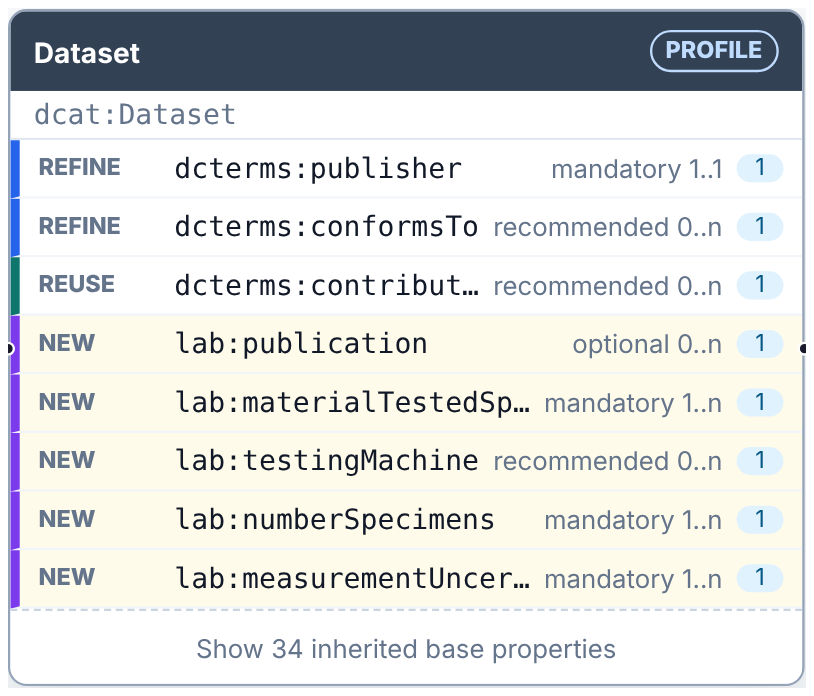
\includegraphics[width=\linewidth]{figures/wb-canvas-dataset.png}\\[0.6ex]
    {\scriptsize (a) Canvas card of \term{dcat:Dataset}}\\[1.2ex]
    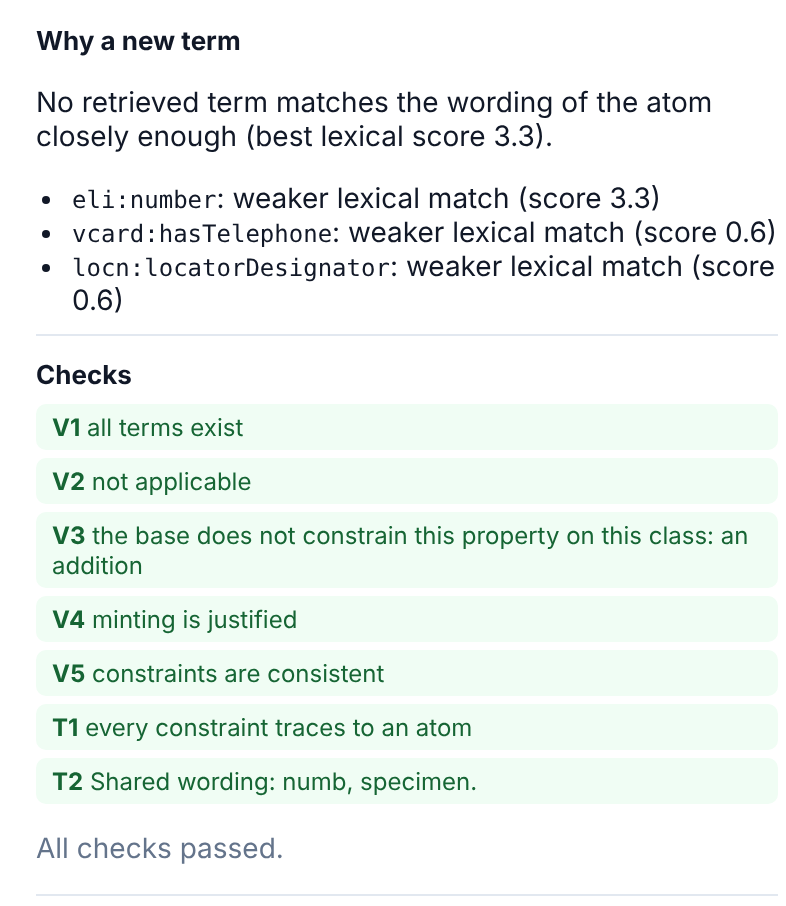
\includegraphics[width=\linewidth]{figures/wb-inspector-mint-bottom.png}\\[0.6ex]
    {\scriptsize (c) Inspector, continued: rejected candidates and checks}
  \end{minipage}\hfill
  \begin{minipage}[t]{0.485\textwidth}
    \vspace{0pt}
    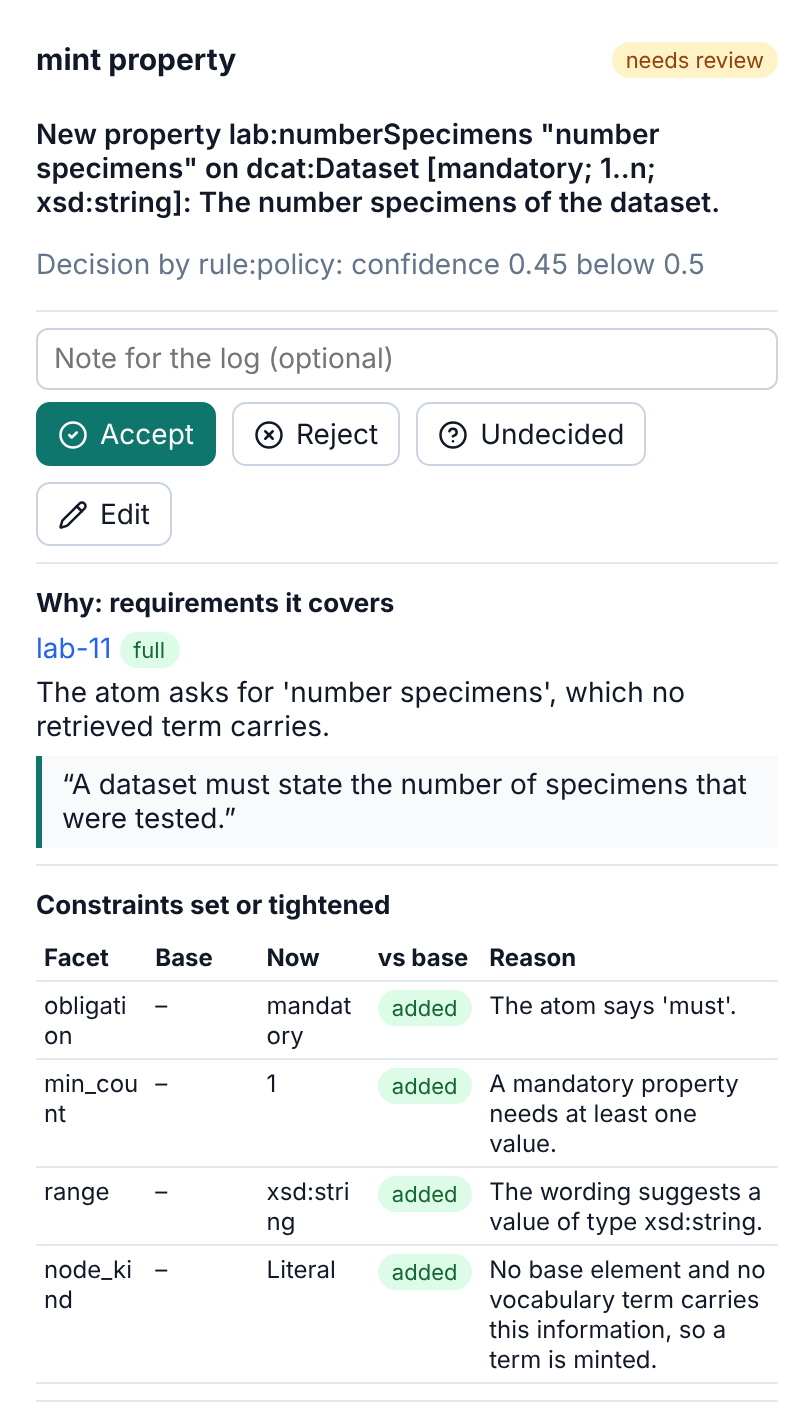
\includegraphics[width=\linewidth]{figures/wb-inspector-mint-top.png}\\[0.6ex]
    {\scriptsize (b) Inspector of one minted property}
  \end{minipage}
  \caption{The workbench on the synthetic demo of Table~\ref{tab:criteria}, run with the offline rules provider
    instead of a model, so the choices shown are a lexical baseline's (\term{xsd:string} for a count).
    (a)~Rows that tighten a base constraint (REFINE), add an existing term (REUSE) or mint one (NEW),
    with obligation, cardinality and atoms covered; shaded rows wait for review. (b)~The decision and why the
    machine left it open, the covered atom with its verbatim quote, and one justification per constraint, with
    base and new value. (c)~The candidates the mint rejected, with their lexical scores, and the checks.}
  \label{fig:workbench}
\end{figure}


\section{The Benchmark in Full}\label{app:benchmark}

Table~\ref{tab:cases-full} lists the cases in full, and Fig.~\ref{fig:reference} shows how a reference delta is built
and matched (Sect.~\ref{sec:benchmark}). \todo{cases in full: base release and reference version per case (Q3);
source of each reference delta (Q23); elements by kind; aligned elements (Q9); A-rq1 (Q21); counterfactual atoms
per case; test-case atom counts as in Table~\ref{tab:cases} (Q11)}

\begin{table}[tp]
  \caption{The five cases in full, test cases above development cases. Base: the release the reference delta is
    computed against. Reference: the published profile and its version; in parentheses, how the reference delta
    is obtained, shapes compared or tables extracted by hand. Elements: reference elements by kind; loosened:
    elements that relax the base, reported apart. Aligned: elements at least one atom asks for (in parentheses,
    those none asks for). Atoms: A-gold, the scored content atoms of the companion benchmark
    \cite{anon2027rq1}; A-rq1, atoms converted from the needs of the companion workflow; counterfactual, atoms
    reworded so that the right answer departs from the publication.}
  \label{tab:cases-full}
  \centering\scriptsize
  \setlength{\tabcolsep}{2.5pt}
  \begin{tabular}{@{}>{\raggedright\arraybackslash}p{1.95cm}>{\raggedright\arraybackslash}p{1.3cm}rrrrrrrrr@{}}
    \toprule
    & & \multicolumn{4}{c}{Elements} & & & \multicolumn{3}{c}{Atoms}\\
    \cmidrule(lr){3-6}\cmidrule(l){9-11}
    Case (base) & Reference (source) & reuse & refine & mint & class & loosened & Aligned & A-gold & A-rq1
      & counterf.\\
    \midrule
    % Base, reference and source: author decisions (Q3, Q23), \tbd here. Counts: \res slots for the RQ2 evaluator
    % (scopes as in Table 2: mobility, geo, health, test, stat, jrc, five; condition "all"); they print \tbd until
    % defined. A-gold: the companion's scored content atoms (RQ1 Table 1, "Atoms").
    mobilityDCAT-AP (\tbd) & \tbd{} (\tbd) & \res{mobility}{all}{reuse} & \res{mobility}{all}{refine} & \res{mobility}{all}{mint} & \res{mobility}{all}{class} & \res{mobility}{all}{loosened}
      & \res{mobility}{all}{N} (\res{mobility}{all}{unaligned}) & 39 % src: RQ1 L382 (Table 1, Atoms)
      & \res{mobility}{all}{arq1} & \res{mobility}{all}{counterfactual}\\
    GeoDCAT-AP (\tbd) & \tbd{} (\tbd) & \res{geo}{all}{reuse} & \res{geo}{all}{refine} & \res{geo}{all}{mint} & \res{geo}{all}{class} & \res{geo}{all}{loosened}
      & \res{geo}{all}{N} (\res{geo}{all}{unaligned}) & 37 % src: RQ1 L383
      & \res{geo}{all}{arq1} & \res{geo}{all}{counterfactual}\\
    HealthDCAT-AP (\tbd) & \tbd{} (\tbd) & \res{health}{all}{reuse} & \res{health}{all}{refine} & \res{health}{all}{mint} & \res{health}{all}{class} & \res{health}{all}{loosened}
      & \res{health}{all}{N} (\res{health}{all}{unaligned}) & 89 % src: RQ1 L384
      & \res{health}{all}{arq1} & \res{health}{all}{counterfactual}\\
    \textit{Test cases} &  & \res{test}{all}{reuse} & \res{test}{all}{refine} & \res{test}{all}{mint} & \res{test}{all}{class} & \res{test}{all}{loosened}
      & \res{test}{all}{N} (\res{test}{all}{unaligned}) & 165 % src: RQ1 L385 (39+37+89)
      & \res{test}{all}{arq1} & \res{test}{all}{counterfactual}\\
    \midrule
    StatDCAT-AP (\tbd) & \tbd{} (\tbd) & \res{stat}{all}{reuse} & \res{stat}{all}{refine} & \res{stat}{all}{mint} & \res{stat}{all}{class} & \res{stat}{all}{loosened}
      & \res{stat}{all}{N} (\res{stat}{all}{unaligned}) & 14 % src: RQ1 L386
      & \res{stat}{all}{arq1} & \res{stat}{all}{counterfactual}\\
    DCAT-AP-JRC (\tbd) & \tbd{} (\tbd) & \res{jrc}{all}{reuse} & \res{jrc}{all}{refine} & \res{jrc}{all}{mint} & \res{jrc}{all}{class} & \res{jrc}{all}{loosened}
      & \res{jrc}{all}{N} (\res{jrc}{all}{unaligned}) & 17 % src: RQ1 L387
      & \res{jrc}{all}{arq1} & \res{jrc}{all}{counterfactual}\\
    \midrule
    All five &  & \res{five}{all}{reuse} & \res{five}{all}{refine} & \res{five}{all}{mint} & \res{five}{all}{class} & \res{five}{all}{loosened}
      & \res{five}{all}{N} (\res{five}{all}{unaligned}) & 196 % src: RQ1 L388 (165+14+17)
      & \res{five}{all}{arq1} & \res{five}{all}{counterfactual}\\
    \bottomrule
  \end{tabular}
\end{table}

\begin{figure}[tp]
  \centering
  % Fig. 4: from a published profile to Recovery (appendix B). Mirrors the RQ1 paper's Fig. 4: seven numbered steps
% in a zigzag (1-3 left to right, 4-6 right to left, 7 below), the final box filled, and a dashed path from the steps
% that set elements apart into a dashed box for what stays outside the denominator. Node and arrow styles follow
% figures/pipeline.tex. Box texts: outline-final.md, brief 6.10 (Fig. 4). Input inside a figure environment
% (sections/11-appendix.tex), which holds the caption and the label fig:reference.
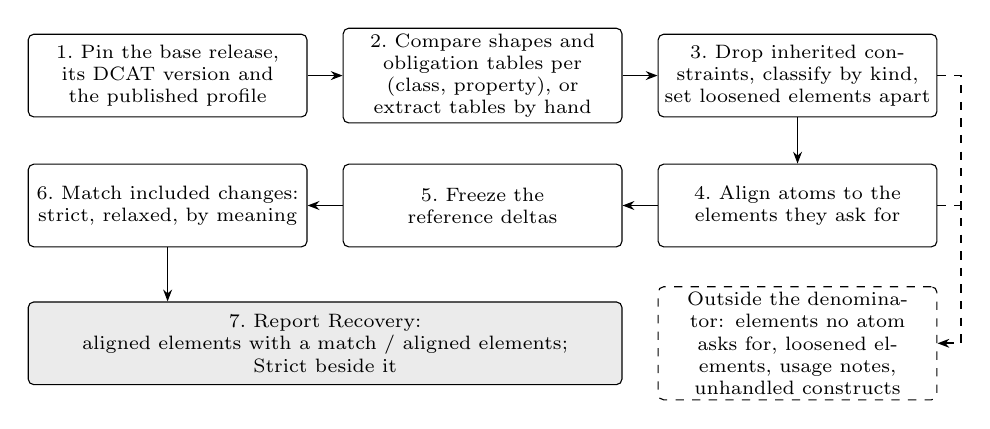
\begin{tikzpicture}[
    font=\scriptsize,
    op/.style={draw, rounded corners=2pt, minimum height=1.05cm, align=center,
               inner sep=2pt, text width=3.4cm},
    final/.style={op, fill=black!8, text width=7.4cm},
    outside/.style={op, dashed},
    flow/.style={-{Stealth[length=1.5mm]}, semithick},
    side/.style={-{Stealth[length=1.5mm]}, semithick, dashed},
  ]
  % row 1: build the reference delta (left to right)
  \node[op] (s1) at (0,0)   {1.\ Pin the base release, its DCAT version and the published profile};
  \node[op] (s2) at (4,0)   {2.\ Compare shapes and obligation tables per (class, property), or extract tables by hand};
  \node[op] (s3) at (8,0)   {3.\ Drop inherited constraints, classify by kind, set loosened elements apart};
  % row 2: fix the denominator, then match (right to left)
  \node[op] (s4) at (8,-1.65) {4.\ Align atoms to the\\ elements they ask for};
  \node[op] (s5) at (4,-1.65) {5.\ Freeze the\\ reference deltas};
  \node[op] (s6) at (0,-1.65) {6.\ Match included changes:\\ strict, relaxed, by meaning};
  % row 3: the report (filled) and what stays outside the denominator (dashed)
  \coordinate (r3) at (0,-3.4);
  \node[final, anchor=west] (s7) at (s6.west |- r3)
        {7.\ Report Recovery:\\ aligned elements with a match / aligned elements;\\ Strict beside it};
  \node[outside] (out) at (8,-3.4)
        {Outside the denominator: elements no atom asks for, loosened elements, usage notes, unhandled constructs};
  % solid path
  \draw[flow] (s1) -- (s2);
  \draw[flow] (s2) -- (s3);
  \draw[flow] (s3) -- (s4);
  \draw[flow] (s4) -- (s5);
  \draw[flow] (s5) -- (s6);
  \draw[flow] (s6.south) -- (s6.south |- s7.north);
  % dashed path: elements set apart in step 3 and left unaligned in step 4
  \coordinate (bus) at ([xshift=3mm]s3.east);
  \draw[side] (s3.east) -- (bus) |- (out.east);
  \draw[semithick, dashed] (s4.east) -- (s4.east -| bus);
\end{tikzpicture}

  \caption{From a published profile to Recovery, in the order of the arrows. Steps 1 to 5 fix the denominator,
    the aligned reference elements, before step 6 matches any output; the dashed path collects what stays
    outside it. Strict is reported beside Recovery.}
  \label{fig:reference}
\end{figure}


\end{document}
